\documentclass[
    14pt, 
    a4paper, 
    titlepage, 
    fleqn
]{extarticle}

\usepackage{style/style}
\usepackage{style/titlepage}
\usepackage{style/math}

\begin{document}

    \fefutitlepageVKR{
    Держапольский Юрий Витальевич
}{
    МОДЕЛИРОВАНИЕ ТРОФИЧЕСКИХ СЕТЕЙ
    \vspace{-10pt}

    (Особенности динамики видов в трофических цепях)
}{
    01.03.02 <<Прикладная математика и информатика>>
}

\fefureverseVKR{
    проф. д.ф.-м.н.
}{
    Абакумов А. И.
}{
    3
}{
    4
}
    
    \tableofcontents

    \pagebreak

    \section{Введение}
    В Дальневосточном Федеральном Университете ведётся учёт картриджей для оборудования для печати. Для этого используется подсистема <<1С Предприятия>>, которая содержит все данные об оборудовании, картриджах, их движениях и состояниях. Также с помощью неё регулируются процессы по замене картриджей, их заправки, списания и т.д. Однако, иногда при отправке заявки по замене картриджа могут создаваться дубликаты заявок, например, по случайности или из-за неправильного заполнения данных, поэтому их нужно удалять. Но самостоятельная очистка может занимать много времени, поскольку бизнес процесс, регулирующий это, может иметь несколько задач, которые также требуют удаления.

    Для ускорения этого процесса поставлена задача разработки внешней обработки, которая позволит указывать только бизнес процесс и помечать на удаление все связанные документы и задачи.
    
    \pagebreak

    \section{Математические модели}
    \subsection{Экологическое введение}
    В экологии структура сообщества, демонстрирующая перенос энергии, заключённой в пище от одного вида к другому, где виды связаны между собой отношениями хищник-жертва, называется \textit{трофической цепью}. При каждом очередном переносе значительная часть энергии (\( \approx \)70-80\%) теряется, расходуясь на дыхание и переходя в тепло. Обычно такие потери энергии ограничивают число <<звеньев>> цепи обычно до четырёх-пяти. В существующие цепи могут занестись извне новые виды особей, которые могли бы образовать следующий трофический уровень. В результате увеличения количества энергии, поступающей в систему, или в результате каких-либо воздействий (например, внесения удобрений) значительно возрастает продуктивность первого уровня, вследствие чего может возникнуть и закрепиться новый трофический уровень, обусловленный имеющимся генерационным материалом.
    
    Трофические цепи обычно не изолированы друг от друга, а переплетаются и образуют трофический граф (трофическую сеть). Примером такой трофической сети может послужить экосистема небольшого ручья\cite{jones_river}, изображённая на рис. \ref{small_river_graph}.
    Это открытая экосистема, часть основного ресурса в которую поступает в виде опавших листьев \textit{1} и других органических остатков \textit{2}, приносимых течением. Она включает три трофических уровня. Виды \textit{3} -- зеленые водоросли и \textit{4} -- диатомовые водоросли -- образуют уровень продуцентов; виды \textit{5} -- веснянка, \textit{6} -- поденки и комары-дергуны, \textit{7} -- ручейники и \textit{8} -- поденка (\textit{Ecdyonurus}) -- уровень первичных консументов, а виды \textit{5} -- веснянка (\textit{Perla}) и \textit{12} -- ручейник (\textit{Dinocras}) -- уровень вторичных консументов. Формы 9 -- ручейники, строящие ловчую сеть, -- и \textit{10} -- ручейник (\textit{Rhyacophila}) -- занимают некоторый промежуточный уровень. Здесь можно выделить много последовательностей видов, образующих трофические цепи, например: \(3 \to 6 \to 12\) или \( 2 \to 7 \to 11 \). 

    \begin{figure}[H]
        \centering
        \begin{tikzpicture}
            \usetikzlibrary{shapes.multipart}
    
            \tikzstyle{roundnode} = [draw, circle, text centered,text width=5mm];
            \tikzstyle{squarenode} = [draw, regular polygon, regular polygon sides=4, text centered, inner sep=0];
            \tikzstyle{arrow} = [thick, -{Stealth[length=4mm]}];
            \tikzstyle{arrow2} = [thick, {Stealth[length=4mm]}-{Stealth[length=4mm]} ];

            \node[roundnode] (1) at (0,0) {$1$};
            \node[roundnode] (2) at (5.5,0) {$2$};
            \node[roundnode] (3) at (1.75,-3) {$3$};
            \node[roundnode] (4) at (9,-3) {$4$};
            \node[roundnode] (5) at (0,-6) {$5$};
            \node[roundnode] (6) at (4.5,-6) {$6$};
            \node[roundnode] (7) at (7.5,-6) {$7$};
            \node[roundnode] (8) at (10,-6) {$8$};
            \node[roundnode] (9) at (3,-9) {$9$};
            \node[roundnode] (10)at (8,-9) {$10$};
            \node[roundnode] (11)at (2,-12) {$11$};
            \node[roundnode] (12)at (6,-12) {$12$};

            \draw[arrow] (1) to (5);
            \draw[arrow] (1) to[bend left=16] (6);
            \draw[arrow] (1) to (8);
            \draw[arrow] (1) to (9);

            \draw[arrow] (2) to (6);
            \draw[arrow] (2) to (7);
            \draw[arrow] (2) to (8);

            \draw[arrow] (3) to (6);
            \draw[arrow] (3) to (9);
            \draw[arrow] (3) to (11);

            \draw[arrow] (4) to (6);
            \draw[arrow] (4) to (7);
            \draw[arrow] (4) to (8);
            \draw[arrow] (4) to (9);

            \draw[arrow] (5) to (11);

            \draw[arrow] (6) to (9);
            \draw[arrow] (6) to (10);
            \draw[arrow] (6) to[bend left=16] (11);
            \draw[arrow] (6) to (12);

            \draw[arrow] (7) to[bend left=8] (11);
            \draw[arrow] (7) to (12);

            \draw[arrow] (8) to (10);
            \draw[arrow] (8) to[bend left=20] (12);


            \node (3in) at ([yshift=5cm]3) {};
            \draw[arrow, dashed] (3in) to (3);
            
            \node (4in) at ([yshift=5cm]4) {};
            \draw[arrow, dashed] (4in) to (4);

            \node at (5.5,1.5) {\textit{Солнечный свет}};

            \node (1in) at ([xshift=-3cm]1) {};
            \node (2in) at ([xshift=8cm]2) {};
            
            \draw[arrow] (1in) to (1);
            \draw[arrow] (2in) to node[pos=0.25,anchor=south] {\textit{Вносимая органика}} (2);

            \node at ([xshift=3cm]4) {\textit{Продуценты}};
            \node[align=center] at ([xshift=2cm]8) {\textit{Первичные}\\\textit{консументы}};
            \node[align=center] at ([xshift=4cm]10) {\textit{Промежуточный}\\\textit{уровень}};
            \node[align=center] at ([xshift=5cm]12) {\textit{Вторичные}\\\textit{консументы}};
    
        \end{tikzpicture}
        \caption{Часть трофической сети экосистемы ручья в Южном Уэльсе.} \label{small_river_graph}
    \end{figure}

    Можно сказать, что трофическая цепь описывает сообщество, два последовательных вида которого образуют пару хищник -- жертва. Трофическая цепь начинается с некоторого ресурса.

    Поскольку реальное сообщество описывается достаточно сложной трофической цепью, то и модель усложняется. Есть два пути упрощения исходной модели. Первый это агрегация всех видов, принадлежащих одному и тому же трофическому уровню в один <<псевдовид>>, в случае достаточно близких экологических характеристик видов уровней. Второй это выделение в трофической сети одной вертикальной ветви поток энергии, который намного превосходит потоки энергии по другим ветвям, и пренебрежение остальными, в случае присутствия доминантного вида. В любом случае после таких упрощений на каждом из уровней останется один вид, а трофическая структура этого сообщества будет описываться трофической цепью. В случае невозможности осреднения или выделения доминантной ветви, необходимо будет рассматривать несколько трофических цепей или ветвящиеся трофические цепи.

\subsection{Неветвящиеся трофические цепи}
<<Ресурс>> в реальных экосистемах можно разделить на два вида:
\begin{itemize}
    \item Энергия, например, солнечный свет. Тогда экосистема с данным ресурсом является незамкнутой, и энергия <<протекает>> через систему, в ходе этого рассеиваясь в виде тепла.
    \item Биологические вещества, например, углерод, азот, фосфор. В этом случае экосистема является замкнутой по отношению к ресурсам. Достигается это деятельностью так называемых <<разлагателей>>, которые разлагают мёртвую органику до необходимых минеральных компонентов, необходимых первичным уровням трофической цепи.
\end{itemize}

Соответственно будем рассматривать два типа трофической цепей: незамкнутые (<<проточные>>) и замкнутые (<<циклы>>). Схематически оба эти типа изображены на рис. \ref{shemas}.

Рост и развитие экосистем во многих системах лимитируется каким-либо фактором (\textit{принцип Либиха}). Опять же, например, солнечный свет -- это невозобновимый ресурс и цепь является незамкнутой, а химические вещества за счёт разлагателей снова вовлекаются в деятельность замкнутой экосистемы.

Рассмотрим подробнее схемы на рис. \ref{shemas}. Здесь \(R\) -- ресурс, используемый \(1\)-м видом с биомассой \(N_1\). Удельная скорость использования \(V_0(R)\) -- это количество ресурса, потребляемое единицей биомассы (одной особью) \(1\)-го вида за единицу времени. Из общего количества потребляемого ресурса \(V_0(R)\) только \(k_1\)-доля его идёт на воспроизводство новой биомассы первого вида, остальное расходуется на поддержание жизнедеятельности. Кроме того, с постоянной скоростью \(m_1\) биомасса \(1\)-го вида отмирает. Далее, \(2\)-й вид использует уже в качестве ресурса биомассу \(1\)-го вида, потребляя её с удельной скоростью \(V_1(N_1)\), и т.д. Цепочка заканчивается на \(n\)-м виде, биомассу которого уже никто не потребляет, и он только отмирает со скоростью \(m_n\).

\begin{figure}[H]
\centering
\begin{tikzpicture}

    \usetikzlibrary{shapes.geometric, calc}

    \tikzstyle{roundnode} = [draw, circle, text centered];
    \tikzstyle{squarenode} = [draw, regular polygon, regular polygon sides=4, text centered, inner sep=0];
    \tikzstyle{arrow} = [thick, ->, >=stealth];

    % Left - Flow
    \node[roundnode] (RF) at (0,8) {$R$};

    \node[squarenode] (NF1) at (0,6) {$N_1$};
    \node (NF1M) at (2,6) {$m_1 N_1$};
    \draw [arrow] (NF1) -- (NF1M);

    \node[squarenode] (NF2) at (0,4) {$N_2$};
    \node (NF2M) at (2,4) {$m_2 N_2$};
    \draw [arrow] (NF2) -- (NF2M);

    \node (DF) at (0,2) {$\vdots\vphantom{lp}$};

    \node[squarenode] (NFN) at (0,0) {$N_n$};
    \node (NFNM) at (2,0) {$m_n N_n$};
    \draw [arrow] (NFN) -- (NFNM);


    \draw [arrow] (0,10) -- node[anchor=east] {$Q$} (RF);
    \draw [arrow] (RF) --   node[anchor=east] {$V_0(R)$} (NF1);
    \draw [arrow] (NF1) --  node[anchor=east] {$V_1(N_1)$} (NF2);
    \draw [arrow] (NF2) --  node[anchor=east] {$V_2(N_2)$} (DF);
    \draw [arrow] (DF) --   node[anchor=east] {$V_{n-1}(N_{n-1})$} (NFN);


    \path[arrow] (NF1) edge [loop left] node {$k_1 V_0$} ();
    \path[arrow] (NF2) edge [loop left] node {$k_2 V_1$} ();
    \path[arrow] (NFN) edge [loop left] node {$k_n V_{n-1}$} ();
    % Left - Flow
    
    % Right - Cycle
    \node (BTC) at (11, 10) {};
    \node (BBC) at (11, 0) {};

    \node[roundnode] (RC) at (8,8) {$R$};

    \node[squarenode] (NC1) at (8,6) {$N_1$};
    \draw [arrow] (NC1) -- node[anchor=south] {$m_1 N_1$} ($(BTC)!(NC1)!(BBC)$);

    \node[squarenode] (NC2) at (8,4) {$N_2$};
    \draw [arrow] (NC2) -- node[anchor=south] {$m_2 N_2$} ($(BTC)!(NC2)!(BBC)$);

    \node (DC) at (8,2) {$\vdots\vphantom{lp}$};
    \node (DC2) at ($(BTC)!(DC)!(BBC)$) {$\vdots\vphantom{lp}$};

    \node[squarenode] (NCN) at (8,0) {$N_n$};
    \draw [arrow] (NCN) -- node[anchor=south] {$m_n N_n$} ($(BTC)!(NCN)!(BBC)$);


    \draw [arrow] (8,10) -- node[anchor=east] {$Q$} (RC);
    \draw [arrow] (RC) --   node[anchor=east] {$V_0(R)$} (NC1);
    \draw [arrow] (NC1) --  node[anchor=east] {$V_1(N_1)$} (NC2);
    \draw [arrow] (NC2) --  node[anchor=east] {$V_2(N_2)$} (DC);
    \draw [arrow] (DC) --   node[anchor=east] {$V_{n-1}(N_{n-1})$} (NCN);
    
    \draw [arrow] (DC2) |- node[pos=0.75, anchor=south] 
    {$\textstyle\sum\limits_{i=1}^n a_i m_i N_i$} (RC);


    \path[arrow] (NC1) edge [loop left] node {$k_1 V_0$} ();
    \path[arrow] (NC2) edge [loop left] node {$k_2 V_1$} ();
    \path[arrow] (NCN) edge [loop left] node (KNVN1) {$k_n V_{n-1}$} ();

    \draw [arrow] ($(KNVN1)!(BTC)!(NCN)$) -- (DC2);
    % Right - Cycle

    \node at (0,-1) {\textit{а)}};
    \node at (8,-1) {\textit{б)}};

\end{tikzpicture}
\caption{Схема трофической цепи длины \(n\): a) незамкнутая (<<проточная>>) цепь; б) замкнутая цепь (<<цикл>>). Коэффициенты \(a_i (0 \leq a_i \leq 1)\) -- доли восстановленного видами-разлагателями ресурса, содержащегося в отмершей биомассе \(i\)-го вида.} \label{shemas}
\end{figure}

Вторая схема отличается от первой наличием условного дополнительного вида -- разлагателя -- который в качестве ресурса использует мёртвую биомассу остальных \(n\) видов и за счёт его жизнедеятельности частично восполняет убыль ресурса \(R\). При этом мы будем полагать, что этот вид может практически мгновенно разлагать любое количество биомассы, что восполненный ресурс сразу становится доступен \(1\)-му виду. То есть, нет необходимости рассматривать численность биомассы разлагателя.

Предположим, что экосистема, имеющая трофический граф типа изображённых на рис. \ref{shemas}, стремится к некоторому состоянию равновесия, причём в этом состоянии отличны от нуля стационарные численности только первых \(q\) видов. Такое равновесие будем называть \textit{трофической цепью длины \(q\)}. 

Пусть скорость поступления в экосистему внешнего ресурса равна \(Q\). Тогда будем исследовать какой должна быть эта скорость при заданных функциях и параметрах, чтобы в таком сообществе существовало устойчивое равновесное состояние с ненулевыми численностями первых \(q\) видов. Другими словами, каковы условия существования трофической цепи длины \(q\)?

По трофическим графам \ref{shemas} можно построить следующие системы дифференциальных уравнений. 

\begin{enumerate}[label={\asbuk*)}, ref=\asbuk*]
    \item \textit{Незамкнутая цепь:}
    \begin{equation}  \label{flow_full}
        \begin{split}
            & \frac{dR}{dt} = Q - V_0(R) N_1, \\
            & \frac{dN_1}{dt} = -m_1 N_1 + k_1 V_0(R) N_1 - V_1(N_1) N_2, \\
            & \frac{dN_i}{dt} = -m_i N_i + k_i V_{i-1}(N_{i-1}) N_i - V_i(N_i) N_{i+1}, \quad i=\overline{2,n-1}, \\
            & \frac{dN_n}{dt} = -m_n N_n + k_n V_{n-1}(N_{n-1}) N_n.
        \end{split}
    \end{equation}

    \item \textit{Замкнутая цепь:}
    \begin{equation} \label{cycle_full}
        \begin{split}
            & \frac{dR}{dt} = Q - V_0(R) N_1  + \sum_{i=1}^{n} a_i m_i N_i, \\
            & \frac{dN_1}{dt} = -m_1 N_1 + k_1 V_0(R) N_1 - V_1(N_1) N_2, \\
            & \frac{dN_i}{dt} = -m_i N_i + k_i V_{i-1}(N_{i-1}) N_i - V_i(N_i) N_{i+1}, \quad i=\overline{2,n-1}, \\
            & \frac{dN_n}{dt} = -m_n N_n + k_n V_{n-1}(N_{n-1}) N_n.
        \end{split}
    \end{equation}
\end{enumerate}

По биологическому смыслу параметры $k_i$ и $a_i$ удовлетворяют ограничениям $ 0 \leq k_i, a_i \leq 1 $. Также понятно, что биомасса не может быть отрицательной: \(N_i \geq 0 ~ \forall i\).

Если считать, что ни один вид не имеет в избытке трофического ресурса, т.е. трофические связи <<напряжены>> (почти все жертвы становятся добычей для хищника, который всегда голоден и насыщения не наступает), то в этом случае
\begin{equation}
    V_0(R) = \alpha_0 R, \quad V_i(N_i) = \alpha_i N_i \quad (i=\overline{1,n})
\end{equation}
и уравнения (\ref{flow_full}) и (\ref{cycle_full}) переходят в уравнения вольтерровского типа, за исключением первых уравнений, содержащих слагаемое \(Q\). Тогда, формально полагая \(R \equiv N_0\) и \( N_{n+1} \equiv 0 \), получим две системы, которые описывают динамику двух трофических цепей.  

\begin{enumerate}[label={\asbuk*)}, ref=\asbuk*]
    \item \textit{Незамкнутая цепь:}
    \begin{equation}  \label{flow}
        \begin{split}
            & \frac{dN_0}{dt} = Q - \alpha_0 N_0 N_1, \\
            & \frac{dN_i}{dt} = N_i (-m_i + k_i \alpha_{i-1} N_{i-1}  - \alpha_i N_{i+1}), \quad i=\overline{1,n}.
        \end{split}
    \end{equation}

    \item \textit{Замкнутая цепь:}
    \begin{equation} \label{cycle}
        \begin{split}
            & \frac{dN_0}{dt} = Q - \alpha_0 N_0 N_1  + \sum_{i=1}^{n} a_i m_i N_i, \\
            & \frac{dN_i}{dt} = N_i (-m_i + k_i \alpha_{i-1} N_{i-1}  - \alpha_i N_{i+1}), \quad i=\overline{1,n}.
        \end{split}
    \end{equation}
\end{enumerate}


\subsection{Ветвящиеся трофические цепи}
В реальных экосистемах часто встречается ситуация, когда на каком-то трофическом уровне цепь разветвляется и далее идут уже две или более различные цепи (рис. \ref{schema_split}). 

Пусть разветвление цепи на две происходит на \(s\)-м уровне. Цепь, начинающуюся непосредственно с внешнего ресурса, будем считать \textit{главной} (её длина равна \(q\)), а другую, начинающуюся после ветвления -- \textit{боковой} (её длина равна \(r\)).



\begin{figure}[H]
    \centering
    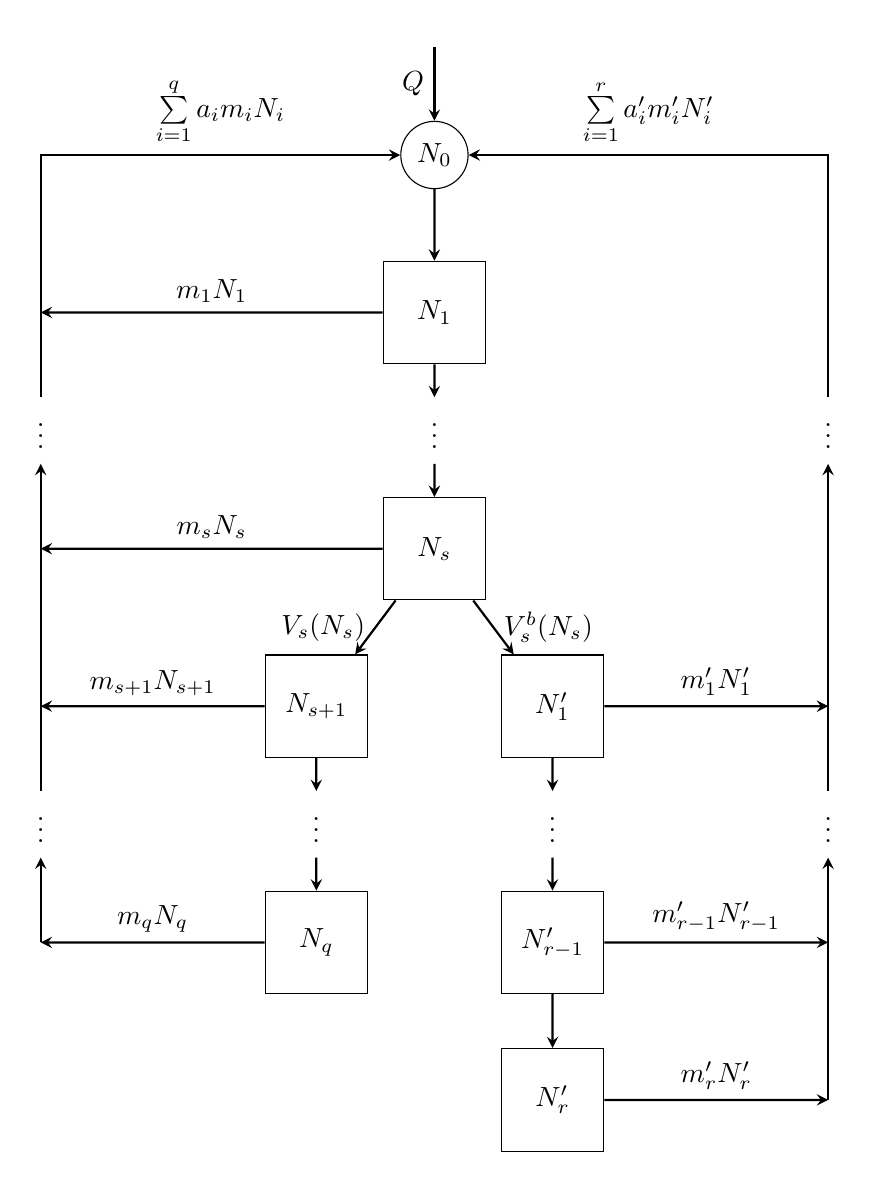
\begin{tikzpicture}

        \usetikzlibrary{shapes.geometric, calc}

        \tikzstyle{roundnode} = [draw, circle, text centered];
        \tikzstyle{squarenode} = [draw, regular polygon, regular polygon sides=4, text centered, inner sep=0, text width=0.92cm];
        \tikzstyle{arrow} = [thick, ->, >=stealth];
        

        \node[roundnode] (N0) at (0,0) {$N_0$};

        \node[squarenode] (N1) at ([yshift=-2cm]N0) {$N_1$};
        \node (ND) at ([yshift=-1.5cm]N1) {$\vdots\vphantom{lp}$};
        \node[squarenode] (NS) at ([yshift=-1.5cm]ND) {$N_s$};


        \node[squarenode] (NS1) at ([xshift=-1.5cm,yshift=-2cm]NS) {$N_{s+1}$};
        \node (NSD) at ([yshift=-1.5cm]NS1) {$\vdots\vphantom{lp}$};
        \node[squarenode] (NQ) at ([yshift=-1.5cm]NSD) {$N_q$};


        \node[squarenode] (M1) at ([xshift=1.5cm,yshift=-2cm]NS) {$N'_{1}$};
        \node (MD) at ([yshift=-1.5cm]M1) {$\vdots\vphantom{lp}$};
        \node[squarenode] (Mm1) at ([yshift=-1.5cm]MD) {$N'_{r-1}$};
        \node[squarenode] (MR) at ([yshift=-2cm]Mm1) {$N'_r$};


        \node (QN0) at ([yshift=1.5cm]N0) {};
        \draw [arrow] (QN0) -- node[anchor=east] {$Q$} (N0);

        
        \draw [arrow] (N0) -- (N1);
        \draw [arrow] (N1) -- (ND);
        \draw [arrow] (ND) -- (NS);
        
        \draw [arrow] (NS) -- node[anchor=east] {$V_s(N_s)$} (NS1);
        \draw [arrow] (NS1) -- (NSD);
        \draw [arrow] (NSD) -- (NQ);

        \draw [arrow] (NS) -- node[anchor=west] {$V^b_s(N_s)$} (M1);
        \draw [arrow] (M1) -- (MD);
        \draw [arrow] (MD) -- (Mm1);
        \draw [arrow] (Mm1) -- (MR);

        \node (DBS) at ([xshift=-5cm]ND) {$\vdots\vphantom{lp}$};
        \node (DBR) at ([xshift=5cm]ND) {$\vdots\vphantom{lp}$};
        \node (DBS2) at ($(DBS)!(NSD)!(DBS)$) {$\vdots\vphantom{lp}$};
        \node (DBR2) at ($(DBR)!(MD)!(DBR)$) {$\vdots\vphantom{lp}$};


        \draw[arrow] ($(DBS)!(NQ)!(DBS)$) -- (DBS2);
        \draw[arrow] (DBS2) -- (DBS);
        \draw[arrow] (DBS) |- node[pos=0.75, anchor=south] {$\textstyle\sum\limits_{i=1}^q a_i m_i N_i$} (N0);


        \draw[arrow] ($(DBR)!(MR)!(DBR)$) -- (DBR2);
        \draw[arrow] (DBR2) -- (DBR);
        \draw[arrow] (DBR) |- node[pos=0.75, anchor=south] {$\textstyle\sum\limits_{i=1}^r a'_i m'_i N'_i$} (N0);


        \draw[arrow] (N1) -- node[anchor=south] {$m_1 N_1$} ($(DBS)!(N1)!(DBS)$);
        \draw[arrow] (NS) -- node[anchor=south] {$m_s N_s$} ($(DBS)!(NS)!(DBS)$);
        \draw[arrow] (NS1) -- node[anchor=south] {$m_{s+1} N_{s+1}$} ($(DBS)!(NS1)!(DBS)$);
        \draw[arrow] (NQ) -- node[anchor=south] {$m_q N_q$} ($(DBS)!(NQ)!(DBS)$);
        

        \draw[arrow] (M1) -- node[anchor=south] {$m'_1 N'_1$} ($(DBR)!(M1)!(DBR)$);
        \draw[arrow] (Mm1) -- node[anchor=south] {$m'_{r-1} N'_{r-1}$} ($(DBR)!(Mm1)!(DBR)$);
        \draw[arrow] (MR) -- node[anchor=south] {$m'_{r} N'_{r}$} ($(DBR)!(MR)!(DBR)$);

    \end{tikzpicture}
    \caption{Схема ветвящейся трофической цепи с двумя ветвями. Виды \(N_i\) -- главная цепь, \(N'_i\) -- боковая.} \label{schema_split}
\end{figure}

По схеме можем построить систему дифференциальных уравнений.
\begin{equation} \label{double_full}
    \begin{split}
        & \frac{d N_0}{dt} = Q - V_0(N_0) N_1 + \sum_{i=1}^q a_i m_i N_i + \sum_{i=1}^r a'_i m'_i N'_i, \\
        & \frac{d N_i}{dt} = -m_i N_i + k_i V_{i-1}(N_{i-1}) N_i - V_i(N_i) N_{i+1}, \quad i=\overline{1,s-1},  \overline{s+1,q}, \\
        & \frac{d N_s}{dt} = -m_s N_s + k_s V_{s-1}(N_{s-1}) N_s - V_s(N_s) N_{s+1} - V_s^b(N_s) N'_1, \\
        & \frac{d N'_1}{dt} = -m'_1 N'_1 + k'_1 V_s^b(N_s) N'_1 - V'_1(N'_1) N'_{2}, \\
        & \frac{d N'_k}{dt} = -m'_k N'_k + k'_k V'_{k-1}(N'_{k-1}) N'_k - V'_k(N'_k) N'_{k+1}, \quad k=\overline{2,r}.
    \end{split}
\end{equation} 
Здесь аналогично \(N_{q+1} \equiv 0, N'_{r+1} \equiv 0\).

    \pagebreak

    \section{Качественная устойчивость}
    Для дальнейшего анализа устойчивости некоторых трофических цепей понадобится определение и критерии свойства под названием \textit{качественная устойчивость}.

    \textit{Вольтеррвоская} модель сообществ \(n\) видов имеет систему вида
    \begin{equation}
        \frac{d N_i}{d t} = N_i \left( \varepsilon_i - \sum_{j=1}^{n} \gamma_{ij} N_j \right), \quad i=\overline{1,n},
    \end{equation}
    где \(\varepsilon_i\) -- скорость естественного прироста или смертности \(i\)-го вида в отсутствие всех остальных видов, а знак и абсолютная величина \(\gamma_{ij} (i \neq j)\) отражают соответственно характер и интенсивность влияния \(j\)-го вида на \(i\)-вид. \(\gamma_{ii}\) -- показатель внутривидового взаимодействия для \(i\)-го вида. Матрицу \(\Gamma = \pares{ \gamma_{ij} } \), отражающую структуру связей сообщества называют \textit{матрицей сообщества}.

    Для описания только характера связей введём \textit{знаковую матрицу} \(S\). Тогда она связана с матрицей сообщества соотношением 
    \[
        S = -\sign \Gamma = \pares{ - \sign \gamma_{ij} }
    \]

    \begin{definition}
        \textbf{Качественная устойчивость сообщества} -- сохранение устойчивости при любых количественных значениях элементов матрицы \(\Gamma = \pares{ \gamma_{ij} }\), сохраняющих лишь тип взаимодействия между каждой парой видов.
    \end{definition}

    Иными словами, качественная устойчивость означает, что сообщество остаётся устойчивым при любых интенсивностях  всех существующих в нем взаимодействий.

    Пусть динамика сообщества \(n\) видов описывается системой уравнений общего вида
    \begin{equation} \label{generic_n}
        \frac{d N_i}{d t} = f_i( \mb{N} ), \quad i = \overline{1,n},
    \end{equation}
    с функциями \(f_i ( \mb{N} )\) допускающими существование равновесия \(N^* > 0\) и линеаризацию в этой точке, то структура соотношений в сообществе может быть определена по матрице системы (\ref{generic_n}), линеаризованной в точке \(N^*\):
    \begin{equation}
        A = \pares{ \left. \frac{\D f_i ( \mb{N} )}{\D N_j} \right|_{N^*} }.
    \end{equation}
    Эта матрица является \textit{матрицей сообщества}. Она описывает характер и интенсивность взаимодействий между видами. Знаковая матрица \(S\) будет равна
    \begin{equation} \label{sign_partial}
        S = \sign A = \pares{ \sign \frac{\D f_i ( \mb{N} )}{\D N_j} }.
    \end{equation}

    Очевидно, что качественная устойчивость является лишь свойством знаковой структуры \(S\) матрицы сообщества \(A\) и на основании (\ref{sign_partial}) может быть сформулирована на языке матриц.
    \begin{definition}
        \textbf{Качественной устойчивостью матрицы} \(A\) (или знак- \hspace{-2pt}устойчивостью) называется устойчивость матрицы \(A\) при любых значениях абсолютных величин её ненулевых элементов.
    \end{definition}
    Иными словами, \(A\) сохраняет устойчивость при любых численных изменениях её элементов, не нарушающих знаковую структуру \(S = \sign A\).

    Если \(A\) не обладает знак-устойчивостью, то в рамках заданной структуры при некотором наборе \({a_{ij}}\) в спектре \(A\) обнаружатся \(\Rez \lambda_i \geq 0\), при этом может существовать такой набор, что матрица окажется устойчивой.

    Для знаковых матриц \(S\) можно указать взаимно однозначное соответствие со \textit{знаковыми ориентированными графами} (далее для краткости ЗОГ). Это получится, если проводить ориентированные рёбра и приписывать им знаки \(+\) или \(-\) по правилу: если вид \(j\) влияет каким-либо образом на вид \(i\), то проводится ребро \(j \to i\) и ему приписывается знак этого влияния.

    Таким образом, условия качественной устойчивости могут формулироваться как в терминах матриц, так и в терминах соответствующих ЗОГ.

\subsection{Необходимые условия}

    Рассмотрим необходимые условия знак-устойчивости матрицы \(A\) \cite{quirk_rupert}:
    \begin{enumerate}
        \item \(a_{ij} a_{ji} \leq 0 \quad \forall i \neq j\); \label{sign_nes_1}
        \item для любой последовательности индексов \(i_1 \neq i_2 \neq i_e \neq \dots i_m \), \(m > 2\) неравенства \(a_{i_1 i_2} \neq 0, a_{i_2 i_3} \neq 0, \dots, a_{i_{m-1} i_m} \neq 0\) влекут \(a_{i_m i_1} = 0\); \label{sign_nes_2}
        \item \(a_{ii} \leq 0 \quad \forall i, \quad \exists i_0 : a_{i_0 i_0} < 0\); \label{sign_nes_3}
        \item существует ненулевой член в разложении \(\det A\). \label{sign_nes_4}
        \item матрица \(A\) является действительной и неразложимой; \label{sign_nes_neraz}
    \end{enumerate}
    С биологической точки зрения эти условия интерпретируются так: (\ref{sign_nes_1}) означает, что в сообществе не должно быть отношений конкуренции или симбиоза. (\ref{sign_nes_3}) означает, что не должно быть самовозрастающих видов и по крайней мере один вид обладает самодемпфированием. Условие (\ref{sign_nes_2}) означает, что ЗОГ сообщества не содержит ориентированных циклов длиной более 2.

    Условие (\ref{sign_nes_4}) формально означает, что есть такая перестановка \(\sigma\) индексов \(1,2,\dots,n\) такая, что произведение элементов \(s_{ij}\) знаковой матрицы \(S = \sign A\) ненулевое:
    \begin{equation} \label{sign_prod}
        s_{1, \sigma(1)} s_{2, \sigma(2)} \cdots s_{n, \sigma(n)} \neq 0.
    \end{equation}

    Известно, что любая перестановка может быть представлена в виде композиции непересекающихся циклов
    \begin{equation*}
        \sigma = c_1 \cdots c_p
    \end{equation*}
    с циклами \(c_j\) длины \(l_j\) такой, что 
    \begin{equation*}
        1 \leq l_j \leq n, \quad \sum_{j=1}^{p} l_j = n.
    \end{equation*}

    Каждому циклу \(c = (i_1, i_2, \dots, i_l)\) длины \(l\) соответствует группа ненулевых сомножителей произведения (\ref{sign_prod}):
    \begin{equation*}
        a_{i_1 i_2} \neq 0, \, a_{i_2 i_3} \neq 0, \, \dots, \, a_{i_{l-1} i_{l}} \neq 0, \, a_{i_l i_1} \neq 0.
    \end{equation*}
    Это соответствует тому, что в ЗОГ вершины \(i_1, \dots, i_l\) соединены в ориентированный цикл. В итоге, условие (\ref{sign_nes_4}) означает, что существует хотя бы одно разбиение ЗОГ на непересекающиеся циклы, сумма длин которых равна \(n\).

    Можно отметить, что учитывая условие (\ref{sign_nes_2}), запрещающее циклы длиннее 2, и (\ref{sign_nes_1}), в ЗОГ качественно устойчивого сообщества можно выделить \(k\) \( \left( 0 \leq k \leq \frac{n}{2} \right)\) пар видов хищник-жертва так, чтобы остальные \(n - 2k\) видов были самодемпфируемыми (являясь циклами длины 1).

    Существенным моментом является условие (\ref{sign_nes_neraz}), которое требует \textit{неразложимость} матрицы. 

    \begin{definition}
        Матрица \(A\) называется \textbf{разложимой}, если некоторой перестановкой её рядов (строк и соответствующих столбцов) она может быть приведена к виду
        \begin{equation}
            A = \pares{ \begin{matrix}
                B & 0 \\
                C & D
            \end{matrix} },
        \end{equation}
        где \(B\) и \(D\) -- квадратные матрицы порядков \(p\) и \(q\) \((p+q = n)\).
    \end{definition}

    Для сообщества неразложимость означает, что в нём нельзя выделить группу \(p\) \( (1 \leq p \leq n)\) видов так, чтобы они не испытывали никакого влияния со стороны остальных \(n-p\) видов. На языке графов это означает, что невозможно выбрать \(p\) вершин так, чтобы ни одна из них не служила концом стрелок, идущих от каких-либо из остальных \(n-p\) вершин. Для матриц это условие требует, чтобы в каждой строке и каждом столбце должен быть хотя бы один ненулевой недиагональный элемент.

    Для примера существенности неразложимости возьмём граф на рис. \ref{example_sign_zog_3}, который соответствует разложимой матрице
    \begin{equation}
        \pares{ \begin{matrix}
            -a & b & c \\
            0 & 0 & -d \\
            0 & e & 0 
        \end{matrix} }, 
        \quad a, b, c, d, e > 0.
    \end{equation}
    Для этого ЗОГ выполняются условия (\ref{sign_nes_1})--(\ref{sign_nes_4}), но он имеет в спектре пару мнимых чисел \(\lambda_{1,2} = \pm i \sqrt{de} ~~ (\lambda_3 = -a)\), т.е. не является устойчивой.
    
    \begin{figure}[H]
        \centering
        \begin{tikzpicture}
    
            \tikzstyle{roundnode} = [draw, circle, text centered];
            \tikzstyle{squarenode} = [draw, regular polygon, regular polygon sides=4, text centered, inner sep=0];
            \tikzstyle{arrow} = [thick, -{Stealth[length=4mm]}];
            \tikzstyle{arrow2} = [thick, {Stealth[length=4mm]}-{Stealth[length=4mm]} ];

            \node[roundnode] (1) at (0,1.5) {$1$};
            \node[roundnode] (2) at (3,3) {$2$};
            \node[roundnode] (3) at (3,0) {$3$};

            \draw [arrow2] (2) -- node[pos=0.1, anchor=west] {$-$} node[pos=0.9, anchor=west] {$+$} (3);
            \draw [arrow] (3) -- node[pos=0.9, anchor=north] {$+$} (1);
            \draw [arrow] (2) -- node[pos=0.9, anchor=south] {$+$} (1);

            \draw[arrow] (1) edge [out=150, in=-150, looseness=8] node [pos=0.9, anchor=north] {$-$} (1);
    
        \end{tikzpicture}
        \caption{Самолимитируемый вид-комменсал \(1\) (питается другим видом без вреда) связан с парой хищник--жертва \(3\)--\(2\).} \label{example_sign_zog_3}
    \end{figure}

    Условие неразложимости ещё более сужает разнообразие видовых соотношений. Этот факт получается из следующей леммы. Для этого введём понятия: матрица \(A\) обладает \textit{симметричной структурой}, если \(\forall i \neq j : a_{ij} \neq 0 \Rightarrow a_{ji} \neq 0 \), и \textit{ассиметричной структурой}, если \(\exists i \neq j : a_{ij} = 0, a_{ji} \neq 0 \).

    \begin{lemma}
        Если \(A\) удовлетворяет условию (\ref{sign_nes_2}) и обладает асимметричной структурой, то \(A\) разложима. \cite{svilog}
    \end{lemma}

    Из этой леммы и условия (\ref{sign_nes_1}) следует, что симметричные ненулевые элементы неразложимой знак-устойчивой матрицы \(A\) должны иметь противоположные знаки, т.е. единственным типом межвидовых отношений в качественно устойчивом сообществе с неразложимой матрицей могут быть лишь отношения хищник--жертва. 

    Рассмотрим сообщество из 5 видов, ЗОГ которого изображён на рис. \ref{example_sign_unstable_zog}, а матрица выглядит так:
    \begin{equation}
        A = \pares{ \begin{matrix}
            0 & 1 & 0 & 0 & 0 \\
            -1& 0 & 1 & 0 & 0 \\
            0 &-1 &-1 & 1 & 0 \\
            0 & 0 &-1 & 0 & 1 \\
            0 & 0 & 0 &-1 & 0
        \end{matrix} }.
    \end{equation}
    
    Как легко убедиться, матрица \(A\) удовлетворяет всем условиям (\ref{sign_nes_1})--(\ref{sign_nes_4}), и, как показывает граф на рисунке \ref{example_sign_unstable_zog}, является неразложимой (\ref{sign_nes_neraz}).

    \begin{figure}[H]
        \centering
        \begin{tikzpicture}
    
            \tikzstyle{roundnode} = [draw, circle, text centered];
            \tikzstyle{squarenode} = [draw, regular polygon, regular polygon sides=4, text centered, inner sep=0];
            \tikzstyle{arrow} = [thick, -{Stealth[length=4mm]}];
            \tikzstyle{arrow2} = [thick, {Stealth[length=4mm]}-{Stealth[length=4mm]} ];

            \node[roundnode] (1) at (0,0) {$1$};
            \node[roundnode] (2) at (3,0) {$2$};
            \node[roundnode] (3) at (6,0) {$3$};
            \node[roundnode] (4) at (9,0) {$4$};
            \node[roundnode] (5) at (12,0) {$5$};

            \draw [arrow2] (1) -- node[pos=0.1, anchor=north] {$+$} node[pos=0.9, anchor=north] {$-$} (2);
            \draw [arrow2] (2) -- node[pos=0.1, anchor=north] {$+$} node[pos=0.9, anchor=north] {$-$} (3);
            \draw [arrow2] (3) -- node[pos=0.1, anchor=north] {$+$} node[pos=0.9, anchor=north] {$-$} (4);
            \draw [arrow2] (4) -- node[pos=0.1, anchor=north] {$+$} node[pos=0.9, anchor=north] {$-$} (5);
            
            \draw[arrow] (3) edge [in=70, out=110, looseness=10] node [pos=0.9, anchor=west] {$-$} (3);
    
        \end{tikzpicture}
        \caption{ЗОГ сообщества 5 видов: \(i\)-й питается \((i+1)\)-м \((i=\overline{1,4})\), при этом \(3\) вид самолимитируется.} \label{example_sign_unstable_zog}
    \end{figure}

    Однако, спектр \(A\) состоит из чисел \(\lambda_1 \approx -0.36\), \(\lambda_{2,3} \approx -0.32 \pm 1.63 i\), \(\lambda_{4,5} = \pm i\), т.е. содержит чисто мнимые числа. Этот пример показывает, что условия (\ref{sign_nes_1})--(\ref{sign_nes_neraz}) являются лишь необходимыми, но не достаточными условиями знак-устойчивости.


\subsection{Достаточные условия} \label{subsec:sign_dost}
    Для получения достаточных условий можно усилить условие (\ref{sign_nes_3}), описывающее самолимитирующие виды \cite{svilog}.

    Для этого определим понятие <<\textit{хищного сообщества}>>. В ЗОГ заданного сообщества рассмотрим какую-нибудь вершину, включенную в цикл длины $2$ ($2$-цикл), одна из стрелок которого имеет знак \(+\), а другая \(-\). Объединим все вершины, которые связаны с данной вершиной такими \(2\)-циклами. Для новых вершин повторяем процедуру объединения с вершинами, связанными с ними теми же \(2\)-циклами. Иными словами, объединим в одно множество все виды, образующие некоторую структуру связей хищник -- жертва. Максимальное множество таких видов будем называть \textbf{хищным сообществом}, содержащим первый вид. Если какой-то вид не связан соотношением \(+ \, -\) ни с какими другими видами, то будем называть его \textit{тривиальным} хищным сообществом.

    ЗОГ на рис. \ref{example_sign_unstable_zog} содержит лишь одно хищное сообщество, включающее все виды. ЗОГ на рис. \ref{example_sign_zog_3} содержит два сообщества: тривиальное \(\{1\}\) и нетривиальное \(\{2,3\}\).

    Разбиению ЗОГ с матрицей \(A = \pares{ a_{ij} } \) на хищные сообщества можно поставить в соответствие матрицу \(\widetilde{A} = \pares{ \widetilde{a}_{ij} } \) по следующему правилу: \(\widetilde{a}_{ij} = a_{ij}\), если ребро \(a_{ij}\) принадлежит некоторому циклу, и \(\widetilde{a}_{ij} = 0\) иначе. Для ЗОГ и матриц, удовлетворяющих условиям (\ref{sign_nes_1}) и (\ref{sign_nes_2}), это означает стирание всех стрелок, связывающих хищные сообщества, а матрица \(A\) приобретает блочно-диагональный вид с блоками, соответствующими отдельным хищным сообществам. Например, для ЗОГ на рис. \ref{example_sign_zog_3} это означает стирание рёбер \(2 \to 1\) и \(3 \to 1\), а матрица \(\widetilde{A}\) принимает вид
    \begin{equation*}
        \widetilde{A} = \pares{ \begin{array}{c|cc}
            -a & 0 & 0 \\ \hline
            0 & 0 & -d \\
            0 & e & 0 
        \end{array} }.
    \end{equation*}

    \begin{lemma} \label{lemma_a_tilde_a}
        Все собственные числа \(A\) и \(\widetilde{A}\) совпадают.
    \end{lemma}

    \begin{proof}
        Пусть элементу \(a_{rs} \neq 0\) соответствует стрелка графа, не принадлежащая никакому циклу (длины больше 1). Это эквивалентно тому, что любое произведение вида
        \begin{equation*}
            a_{rs} a_{sr}, \quad a_{ir} a_{rs} a_{si}, \quad a_{ij} a_{jr} a_{rs} a_{si}, \quad \dots,
        \end{equation*}
        где \(r,s,i,j,dots\) -- различные индексы, обращается в 0 (следует из (\ref{sign_nes_2})).
        Рассмотрим характеристическую матрицу \(\abs{ A - \lambda I } = \abs{ a_{ij} - \delta_{ij} \lambda } \). При её разложении, все члены, содержащие сомножитель \((a_{rs} - \delta_{rs} \lambda)\), исчезнут. То есть, если положить \(a_{rs} = 0\), то значение определителя не изменится. Таким образом,
        \begin{equation*}
            \det \abs{ A - \lambda I } = \det \abs{ \widetilde{A} - \lambda I }.
        \end{equation*}
    \end{proof}

    Значит по устойчивости хищного сообщества можно судить по устойчивости исходного графа. Очевидно, что для устойчивости должно соблюдаться требование 
    \begin{equation*}
        0 \neq \det A = \det \widetilde{A},
    \end{equation*}
    означающее, что все тривиальные хищные сообщества должны обладать самолимитированием.
    
    \begin{theorem} \label{theorem_sign_spectre}
        Если \(A\) удовлетворяет условиям (\ref{sign_nes_1})--(\ref{sign_nes_4}), то \(\Rez \lambda(\widetilde{A}) \leq 0 \), причём кратность значений с нулевой вещественной частью не превосходит \(1\).
    \end{theorem}
    \begin{proof}
        Рассмотрим отдельное хищное сообщество, включающее \(m\) видов, и соответствующую \((m \times m)\)-матрицу \(\widetilde{A}\). Воспользуемся методом Ляпунова для определения устойчивости линейной системы дифференциальных уравнений 
        \begin{equation} \label{sign_hunter_ode}
            \frac{d \mathrm{x}}{dt} = \widetilde{A} \mathrm{x}.
        \end{equation}

        Нужно построить функцию Ляпунова и определить знак её производной по \(t\). Для этого определим \(m\) \textit{положительных чисел} \(\alpha_i\) следующим образом. Положим \(\alpha_1 = 1\). Для каждого \(j\)-го вида, связанного в \(\widetilde{A}\) с \(i\)-м определим соотношение
        \begin{equation} \label{sign_conntcnted_ij}
            \alpha_j a_{ji} = -\alpha_i a_{ij}, \quad i \neq j,
        \end{equation}
        тогда для видов, связанных с \(1\)-м, имеем
        \begin{equation} \label{sign_conntcnted_1}
            \alpha_i = - \frac{a_{1i}}{a_{i1}} > 0
        \end{equation}
        по условию (\ref{sign_nes_1}) и построению хищного сообщества. Поскольку в графе нет замкнутых петель длины больше 2, получим все числа \(\alpha_1, \dots, \alpha_m\).

        Определим функцию
        \begin{equation} \label{sign_lyapunov_func}
            V(x_1, \dots, x_m) = \sum_{i=1}^{m} \alpha_i x_i^2,
        \end{equation}
        где действительный \(m\)-вектор \(\mathrm{x}\) является решением системы (\ref{sign_hunter_ode}). Очевидно, что данная квадратичная форма положительна определена. Найдём её производную на траекториях системы:
        \begin{equation}
            \frac{dV}{dt} = \frac{\D V}{\D \mathrm{x}} \frac{d \mathrm{x}}{dt} = \nabla V \cdot \widetilde{A} \mathrm{x} = \left( 2 \alpha_i x_i \right) \cdot \left( \sum_{j=1}^{m} a_{ij} x_j \right) = 2 \sum_{i=1}^{m} \left( \alpha_i x_i  \sum_{j=1}^{m} a_{ij} x_j \right).
        \end{equation}
        Для каждого слагаемого вида \(\alpha_i a_{ij} x_i x_j\) имеем симметричное \(\alpha_j a_{ji} x_j x_i\) и в силу соотношения (\ref{sign_conntcnted_ij}) они являются противоположными и исчезнут, оставляя только диагональные элементы. Поэтому получаем
        \begin{equation} \label{sign_lyapunov_func_diag}
            \frac{dV}{dt} = 2 \sum_{i=1}^{m} \alpha_i a_{ii} x_i^2 \leq 0,
        \end{equation}
        поскольку \(a_{ii} \leq 0\).

        Функция \(V\) является функцией Ляпунова для нулевого решения системы (\ref{sign_hunter_ode}) поскольку она:
        \begin{enumerate}
            \item непрерывная вместе с частными производными на \( \mbb{R}^m \).
            \item \(V(0, \dots, 0) = 0\);
            \item \( V(x) > 0, x\neq 0 \).
        \end{enumerate}
        Следовательно, по теореме Ляпунова об устойчивости точки равновесия, нулевое решение локально устойчиво. Поэтому \(\Rez \lambda(\widetilde{A}) \leq 0\).
    \end{proof}

    Таким образом, теорема \ref{theorem_sign_spectre} оставляет лишь два возможности для спектра \(\widetilde{A}\): либо все \(\Rez \lambda(\widetilde{A}) < 0\), и нулевое решение асимптотически устойчиво, либо некоторые собственные числа кратности не более \(1\) имеют нулевые вещественные части -- такую ситуацию иногда называют \textit{нейтральной устойчивостью}. Определим условия, которые отделят эти две ситуации.
    
    При \(\det \widetilde{A} \neq 0\) в ситуации нейтральной устойчивости спектр \(\widetilde{A}\) содержит пары чисто мнимых чисел, которым соответствуют синусоидальные (с постоянной амплитудой) слагаемые в общем решении системы (\ref{sign_hunter_ode}). Будем называть компоненты решения \(x_i(t)\), содержащие такие слагаемые, \textit{осциллирующими}.
    
    В структуре хищного сообщества \(\widetilde{A}\) осциллирующие и неосциллирующие виды должны быть расположены специальным образом. 
    \begin{itemize}
        \item Виды \(x_k\) с самолимитированием (\(a_{kk} < 0\)) не могут быть осциллирующими. Это вытекает из того, что периодическому решению системы (\ref{sign_hunter_ode}) соответствует конечная замкнутая траектория в фазовом пространстве и на ней \( \frac{d V}{d t} \equiv 0 \). С учётом (\ref{sign_conntcnted_1}) и (\ref{sign_lyapunov_func_diag}) имеем, что \(x_k \equiv 0\) всюду вдоль периодического решения.
        
        \item Рассмотрим какой-либо осциллирующий вид \(x_i\). Строка системы (\ref{sign_hunter_ode}) этого вида имеет вид
        \begin{equation*}
            \frac{dx_i}{dt} = \sum_{j=1}^{m} a_{ij} x_j.
        \end{equation*}
        В этой строке есть хотя бы один недиагональный ненулевой элемент, который соответствует влиянию другого осциллирующего вида \(x_j\). То есть, осциллирующий вид должен быть связан хотя бы с одним другим осциллирующим видом.

        \item Если неосциллирующий вид связан с некоторым осциллирующим видом, то он с необходимостью имеет связь и с каким-либо другим осциллирующим видом. \cite{svilog}
    \end{itemize}

    Эти требования к структуре нейтрально устойчивого сообщества могут быть формализированы с помощью понятия <<чёрно-белого теста>>. Будем говорить, что хищное сообщество \textit{удовлетворяет чёрно-белому тесту}, если каждая вершина его графа может окрашена в чёрный или белый цвет, что:
    \begin{enumerate}[label={\asbuk*)}, ref=\asbuk*]
        \item все вершины с самолимитированием -- чёрные; \label{black_white_a}
        \item найдётся хотя бы одна белая вершина; \label{black_white_b}
        \item каждая белая вершина связана по крайней мере с одной другой белой вершиной; \label{black_white_c}
        \item каждая чёрная вершина, связанная с белой, связана хотя бы с одной другой белой вершиной. \label{black_white_d}
    \end{enumerate}

        Например, хищное сообщество \(\{1\}\) ЗОГ рис. \ref{example_sign_zog_3} нарушает требование (\ref{black_white_b}), а \(\{ 2, 3 \}\) полностью удовлетворяет тесту. ЗОГ рис. \ref{example_sign_unstable_zog} удовлетворяет тесту, но если переместить самолимитирование в любую другую вершину, тест перестанет выполняться.

        Если хищное сообщество нарушает чёрно-белый тест, то оно не может быть нейтрально устойчивым, и, следовательно, по теореме \ref{theorem_sign_spectre}, оно асимптотически устойчиво. Таким образом, если все хищные сообщества исходного ЗОГ с матрицей \(A\) не удовлетворяют чёрно-белому тесту, то все \(\Rez \lambda(\widetilde{A}) < 0\) и по лемме \ref{lemma_a_tilde_a} матрица \(A\) устойчива.

        В итоге получаем:
        \begin{statement} \label{sign_stab_dost}
            Для качественной устойчивости любой действительной матрицы \(A\) достаточно выполнения совокупности условий (\ref{sign_nes_1}), (\ref{sign_nes_2}), (\ref{sign_dost_3}), (\ref{sign_nes_4}), (\ref{sign_nes_neraz}), где (\labeltext{3'}{sign_dost_3}) требует, чтобы виды с самолимитированием были расположены таким образом, что все его хищные сообщества нарушают чёрно-белый тест (\ref{black_white_a})--(\ref{black_white_d}).
        \end{statement}

    \pagebreak

    \section{Незамкнутые трофические цепи}
    \subsection{Равновесные состояния}
    % Поскольку единственное положительное слагаемое, которое описывает вносимое количество биомассы, в каждой строке зависит от количества биомассы предыдущего вида, то можно сделать вывод, что если в каком-то состоянии равновесия будет вид с нулевой биомассой, то и все последующие виды так же окажутся вымершими.

    % Поэтому в системе (\ref{flow}) при \(Q > 0\) могут существовать \( n \) равновесных состояний типа \(\left[ N_0, N_1, \ldots, N_q, 0, \ldots, 0 \right]\), которые можно определить из уравнений

    Проводится исследование трофических цепей длины \(q\) для системы (\ref{flow}) при \(Q > 0\). То есть устойчивость состояния равновесия вида \(\left[ N_0, N_1, \ldots, N_q, 0, \ldots, 0 \right]\). Корректность данного состояния будет доказана после. Найти это состояние равновесия можно из уравнений
    \begin{equation} \label{flow_stationary_equations}
        \frac{d \mb{N}}{dt} = 0 \Rightarrow
        \left\lbrace\begin{split}
            & N_1 = \frac{Q}{\alpha_0 N_0}, \\
            & \alpha_i N_{i+1} = k_i \alpha_{i-1} N_{i-1} - m_i, \quad i=\overline{1,q}                
        \end{split}\right.
    \end{equation}

    Из условия \( N_{q+1} = 0 \) вытекает, что 
    \begin{equation}
        N_{q-1} = \frac{m_q}{\alpha_{q-1} k_q}.
    \end{equation}

    Отметим, что в уравнениях (\ref{flow_stationary_equations}) есть связь только между \((i+1)\) и \((i-1)\) уравнениями (кроме \(0\) и \(1\)), поэтому формулы вычисления будут зависеть от чётности \(q\).

    Введём обозначения:
    \begin{equation} \label{flow_sub}
        \begin{split}
        & g_i = \frac{k_i \alpha_{i-1}}{\alpha_i}, \quad \mu_i = \frac{m_i}{\alpha_i}, \quad
        H_{2s-1} = g_1 g_3 \cdots g_{2s-1}, \quad H_{2s} = g_2 g_4 \cdots g_{2s}, \\
        & f_{2s-1} = \frac{\mu_1}{H_1} + \frac{\mu_3}{H_3} + \cdots + \frac{\mu_{2s-1}}{H_{2s-1}}, \quad
        f_{2s} = \frac{\mu_2}{H_2} + \frac{\mu_4}{H_4} + \cdots + \frac{\mu_{2s}}{H_{2s}}.
        \end{split}
    \end{equation}

    Последовательно выражая значения \(N_{i}\) имеем
    \begin{equation*}
        \begin{split}
            & N_{i} = \frac{k_{i-1} \alpha_{i-2}}{\alpha_{i-1}} N_{i-2} - \frac{m_{i-1}}{\alpha_{i-1}} = g_{i-1} N_{i-2} - \mu_{i-1} =\\ 
            &= g_{i-1} \left( g_{i-3} N_{i-4} - \mu_{i-3} \right) - \mu_{i-1} = g_{i-1} g_{i-3} N_{i-4} - g_{i-1} \mu_{i-3} - \mu_{i-1} = \dots ;
        \end{split}
    \end{equation*}

    Пусть \(i = 2s\), тогда
    \begin{equation} \label{flow_2s}
        \begin{split}
        & N_{2s} = ( g_{2s-1} g_{2s-3} \cdots g_1 ) N_0 - ( g_{2s-1} \cdots g_3 ) \mu_1 - ( g_{2s-1} \cdots g_5 ) \mu_3 - \cdots - \\
        & - g_{2s-1} \mu_{2s-3} - \mu_{2s-1} = g_{2s-1} \cdots g_1 \left( N_0 - \frac{\mu_1}{g_1} - \dots - \frac{\mu_{2s-1}}{g_1 \cdots g_{2s-1}} \right) = \\
        & = H_{2s-1} \left( N_0 - \frac{\mu_1}{H_1} - \dots - \frac{\mu_{2s-1}}{H_{2s-1}} \right)
        = H_{2s-1} \left( N_0 - f_{2s-1} \right).
        \end{split}
    \end{equation}
    Аналогично получаются значения при \(i = 2s + 1\): 
    \begin{equation} \label{flow_2s1}
        N_{2s+1} = H_{2s} (N_1 - f_{2s}).
    \end{equation}
    Здесь \( s=1,2,\ldots \)

    Для вычисления всех значений не хватает формулы для \(N_0\) или \(N_1\). Отдельно рассмотрим два случая чётности.
    \begin{enumerate}
        \item Пусть \(q = 2s\) -- \textit{чётное}. Тогда
        \begin{equation*}
            N_{q-1} = N_{2s-1} = \frac{m_{2s}}{\alpha_{2s-1} k_{2s}} \frac{\alpha_{2s}}{\alpha_{2s}} = \frac{\mu_{2s}}{g_{2s}}, \quad N_{2s-1} = H_{2s-2} (N_1 - f_{2s-2}).
        \end{equation*}
        Откуда получаем
        \begin{equation*}
            N_1 = \frac{\mu_{2s}}{g_{2s} H_{2s-2}} + f_{2s-2} = \frac{\mu_{2s}}{H_{2s}} + f_{2s-2} = f_{2s}.
        \end{equation*}
        Используя первое уравнение в (\ref{flow_stationary_equations}), будем иметь
        \begin{equation*}
            N_0 = \frac{Q}{\alpha_0 N_1} = \frac{Q}{\alpha_0 f_{2s}}.
        \end{equation*}

        \item Пусть \(q = 2s+1\) -- \textit{нечётное}. Аналогично предыдущему получаем
        \begin{equation*}
            N_{q-1} = N_{2s} = \frac{m_{2s+1}}{\alpha_{2s} k_{2s+1}} \frac{\alpha_{2s+1}}{\alpha_{2s+1}} = \frac{\mu_{2s+1}}{g_{2s+1}}, \quad N_{2s} = H_{2s-1} (N_0 - f_{2s-1}).
        \end{equation*} 
        откуда
        \begin{equation*}
            N_0 = \frac{\mu_{2s+1}}{g_{2s+1} H_{2s-1}} + f_{2s-1} = f_{2s+1}, \quad N_1 = \frac{Q}{\alpha_0 f_{2s+1}}.
        \end{equation*}
    \end{enumerate}

    Теперь легко можно получить явные выражения \(N_i\), подставив \(N_0\) и \( N_1\) в (\ref{flow_2s}) и (\ref{flow_2s1}).

    Очевидно, что стационарные значения численностей \(N_i\) имеют смысл, только когда они положительные.

    \begin{statement}
        Если в \textbf{незамкнутой} трофической цепи длины \(q\) численность \(N_q > 0\), то \(N_i > 0 \, (i=\overline{1,q-1})\).
    \end{statement}

    \begin{proof}
        Для начала заметим, что \(f_{2s}\) и \(f_{2s+1}\) положительны и монотонно возрастают с увеличением \(s\). Величины \(N_0\) и \(N_1\) также положительны и зависят от параметра \(q\) -- длины трофической цепи.  
        Поскольку все параметры положительные, то численность \( N_{q-1} > 0 \).

        Из условия \( N_q > 0 \) и (\ref{flow_2s}, \ref{flow_2s1}) получим неравенство
        \begin{equation} \label{flow_lower}
            Q > \alpha_0 f_{q-1} f_{q}
        \end{equation} 

        Предположим противное: \(\exists p < q : N_p \leq 0\). Возможны 4 варианта: \(p\) и \(q\) одинаковой чётности и разной чётности.

        \begin{enumerate}
            \item Пусть \(q = 2s \) и \( N_0 = \frac{Q}{\alpha_0 f_{2s}}, N_1 = f_{2s}\).
            \begin{enumerate}
                \item \(p = 2u \, (u < s)\), тогда из (\ref{flow_2s}) следует, что \( N_p = N_{2u} \leq 0 \), если \(N_0 \leq f_{2u-1}\). Значит \(Q \leq \alpha_0 f_{2u-1} f_{2s} \). Сравнивая с (\ref{flow_lower}) получаем
                \begin{equation*}
                    \alpha_0 f_{2s-1} f_{2s} < Q \leq \alpha_0 f_{2u-1} f_{2s} \Rightarrow f_{2s-1} < f_{2u-1}.
                \end{equation*}
                Это невозможно, поскольку \(f_{2s-1}\) монотонно возрастает с ростом \(s\).

                \item \(p = 2u+1 \, (2u < 2s-1)\), тогда из (\ref{flow_2s1}) следует, что \( N_p = N_{2u+1} \leq 0 \) при \(N_1 \leq f_{2u}\), т.е. \(f_{2s} \leq f_{2u} \). Что также невозможно из-за монотонного возрастания \(f_{2s}\) с ростом \(s\). 
            \end{enumerate}

            \item Пусть \( q = 2s+1 \) и \( N_0 = f_{2s+1}, N_1 = \frac{Q}{\alpha_0 f_{2s+1}}\).
            \begin{enumerate}
                \item \(p = 2u \, (2u-1 < 2s)\), тогда \( N_p = N_{2u} \leq 0 \) при \(N_0 \leq f_{2u-1}\). Значит \(f_{2s+1} < f_{2u-1} \). 
                
                Это невозможно, поскольку \(f_{2s-1}\) монотонно возрастает с ростом \(s\).

                \item \(p = 2u+1 \, (u < s)\), тогда \( N_p = N_{2u+1} \leq 0 \) при \(N_1 \leq f_{2u}\), т.е. \( Q \leq \alpha f_{2u} f_{2s+1} \). Сравнивая с (\ref{flow_lower}) получаем
                \begin{equation*}
                    \alpha_0 f_{2s} f_{2s+1} < Q \leq \alpha f_{2u} f_{2s+1} \Rightarrow f_{2s} < f_{2u}.
                \end{equation*}
                Что также невозможно из-за монотонного возрастания \(f_{2s}\) с ростом \(s\). 
            \end{enumerate}
        \end{enumerate}
    \end{proof}
    
    \begin{corollary}
        Из (\ref{flow_lower}) следует, что если длина трофической цепи равна \(q\), то скорость поступления ресурса \( Q \) должна превосходить критическое значение 
        \begin{equation*}
            Q^* (q) = \alpha_0 f_{q-1} f_{q}.
        \end{equation*}
    \end{corollary}

\subsection{Условия существования цепи фиксированной длины}

    Для определения устойчивости равновесного состояния трофической цепи длины \(q\): \(N^* = [ N_0, N_1, \dots, N_q, 0, \dots, 0 ]\) будем исследовать собственные значения матрицы системы (\ref{flow}), линеаризованной в окрестности этого состояния.
    
    Найдём матрицу якоби этой системы и подставим равновесную точку: \( \left.\frac{\partial f}{\partial N}\right|_{N^*} \) (\(f\) -- правая часть системы). Получим матрицу
    \begin{equation} \label{flow_jacobian_small}
        J = \left\Vert \begin{matrix}
            A_q & 0 \\
            0 & D_{n-q}
        \end{matrix} \right\Vert,
    \end{equation}
    где \(D_{n-q} = \diag\left\{ -m_{q+1} + k_{q+1} \alpha_q N_q, -m_{q+2}, \ldots, -m_{n} \right\}\) и \(A_q\) матрица вида:
    \begin{equation} \label{flow_jacobian_big}
        A_q = \left\Vert \begin{matrix}
                -b_0  & -d_0   &          &     0    & \\
                b_1  & -h_1   &  -d_1    &          & \\
                        & \ddots & \ddots   &  \ddots  &          \\
                        &        & b_{q-1}  & -h_{q-1} & -d_{q-1} \\
                        &   0    &          & b_{q}    & -h_{q}  
        \end{matrix} \right\Vert
    \end{equation}
    Матрица такого вида принадлежит к классу якобиевых. В нашем случае 
    \begin{equation} \label{flow_jacobian_vars}
        \begin{split}
            & b_0 = \alpha_0 N^*_1, \quad d_0 = \alpha_0 N^*_0, \\
            & b_i = k_i \alpha_{i-1} N^*_i, \quad d_i = \alpha_i N^*_i, \quad h_i = 0, \quad i=\overline{1,q}.
        \end{split}
    \end{equation}
    Значения \(h_i\) следуют из уравнений (\ref{flow_stationary_equations}).


    Собственные значения \(J\) равны
    \begin{equation} \label{flow_jacobian_spectrum}
        \lambda_i = \left\{ \begin{matrix}
            \lambda_i (A_q), & i=\overline{1,q}, \\
            k_{q+1} \alpha_q N_q - m_{q+1}, & i=q+1, \\
            -m_i, & i=\overline{q+2, n}. 
        \end{matrix} \right.
    \end{equation}
    Очевидно, что при \(i = \overline{q+2,n}\) выполняется условие \(\lambda = -m_i < 0\). Для \(\lambda_{q+1}\) все переменные положительные и достаточно выполнения неравенства
    \begin{equation} \label{flow_nq_upper}
        N_q < \frac{m_{q+1}}{\alpha_q k_{q+1}}.
    \end{equation}
    Это условие становится излишним, при \(q = n\), поскольку тогда устойчивость определяется собственными значениями матрицы \(A_q\).

    ЗОГ, соответствующий \(A_q\), имеет вид, изображённый на рис. \ref{example_aq}. Для определения устойчивости матрицы \(A_q\) проверим выполнение достаточных условий знак-устойчивости (\ref{subsec:sign_dost}):
    \begin{enumerate}
        \item все противоположно направленные рёбра имеют противоположные знаки \((a_{ij} a_{ji} < 0)\);
        \item отсутствуют ориентированные циклы длиной более \(2\);
        \item все вершины составляют одно хищное сообщество, нарушающее чёрно-белый тест.
        \item разбиение на циклы, соответствующее ненулевому члену \(\det A_q\) задаётся вершинами:
        \begin{itemize}
            \item \(\{0\}; \{1,2\}; \dots; \{q-1, q\}\), когда \(q\) чётное;
            \item \(\{0, 1\}; \{2,3\}; \dots; \{q-1, q\}\), когда \(q\) нечётное;
        \end{itemize}
        \item никакие вершины не являются концами стрелок, что значит матрица \(A_q\) является неразложимой.
    \end{enumerate}
    
    \begin{figure}[H]
        \centering
        \begin{tikzpicture}
    
            \tikzstyle{roundnode} = [draw, circle, text centered, text width=9mm];
            \tikzstyle{squarenode} = [draw, regular polygon, regular polygon sides=4, text centered, inner sep=0];
            \tikzstyle{arrow} = [thick, -{Stealth[length=4mm]}];
            \tikzstyle{arrow2} = [thick, {Stealth[length=4mm]}-{Stealth[length=4mm]} ];

            \node[roundnode] (0) at (0,0) {$0$};
            \node[roundnode] (1) at (3,0) {$1$};
            \node[roundnode] (2) at (6,0) {$2$};
            \node[roundnode] (q1) at (10,0) {$q-1$};
            \node[roundnode] (q) at (13,0) {$q$};

            \draw [arrow] (1) to[bend right] node[pos=0.9, anchor=south] {$-$} (0);
            \draw [arrow] (0) to[bend right] node[pos=0.9, anchor=north] {$+$} (1);

            \draw [arrow] (2) to[bend right] node[pos=0.9, anchor=south] {$-$} (1);
            \draw [arrow] (1) to[bend right] node[pos=0.9, anchor=north] {$+$} (2);

            \draw [arrow] (q) to[bend right] node[pos=0.9, anchor=south] {$-$} (q1);
            \draw [arrow] (q1) to[bend right] node[pos=0.9, anchor=north] {$+$} (q);

            \node (d_u) at (8, 0.6) {\(\dots\)};
            \node (d_d) at (8,-0.6) {\(\dots\)};
            
            \draw [thick] (q1) to[out=150, in=0] (d_u);
            \draw [arrow] (d_u) to[out=180, in=30] node[pos=0.8, anchor=south] {$-$} (2);
            
            \draw [thick] (2) to[out=-30, in=180] (d_d);
            \draw [arrow] (d_d) to[out=0, in=-150] node[pos=0.8, anchor=north] {$+$} (q1);
            
            \draw[arrow] (0) edge [in=-150, out=150, looseness=6] node [pos=0.9, anchor=north] {$-$} (0);
    
        \end{tikzpicture}
        \caption{ЗОГ, соответствующий матрице \(A_q\) со значениями (\ref{flow_jacobian_vars}).} \label{example_aq}
    \end{figure}

    Таким образом матрица \(A_q\) удовлетворяет достаточным условием знак-устойчивости и поэтому устойчива при любых значениях заданных параметров. А это значит, что равновесие \(N^*\) асимптотически устойчиво.

    Находя явное значение \(N_q\) для чётного и нечётного \(q\) и используя (\ref{flow_nq_upper}) получим:
    \begin{enumerate}
        \item При \(q = 2s\):
        \begin{equation}
            \begin{split}
                & N_{2s} = H_{2s-1} \left( \frac{Q}{\alpha_0 f_{2s}} - f_{2s-1} \right) < \frac{m_{2s+1}}{\alpha_{2s} k_{2s+1}} \Rightarrow \\
                & \Rightarrow \frac{Q}{\alpha_0 f_{2s}} - f_{2s-1} < \frac{m_{2s+1}}{\alpha_{2s} k_{2s+1}} \frac{\alpha_{2s+1}}{\alpha_{2s+1}} \frac{1}{H_{2s-1}} = \frac{\mu_{2s+1}}{g_{2s+1} H_{2s-1}} = \frac{\mu_{2s+1}}{H_{2s+1}} \Rightarrow \\
                & Q < \alpha_0 f_{2s} \left(  f_{2s-1} + \frac{\mu_{2s+1}}{H_{2s+1}} \right) = \alpha_0 f_{2s} f_{2s+1},        
            \end{split}
        \end{equation}
        
        \item При \(q = 2s+1\):
        \begin{equation}
            \begin{split}
                & N_{2s+1} = H_{2s} \left( \frac{Q}{\alpha_0 f_{2s+1}} - f_{2s+1} \right) < \frac{m_{2s+2}}{\alpha_{2s+1} k_{2s+2}} \Rightarrow \\
                & \Rightarrow \frac{Q}{\alpha_0 f_{2s+1}} - f_{2s} < \frac{m_{2s+2}}{\alpha_{2s+1} k_{2s+2}} \frac{\alpha_{2s+2}}{\alpha_{2s+2}} \frac{1}{H_{2s}} = \frac{\mu_{2s+2}}{g_{2s+2} H_{2s}} = \frac{\mu_{2s+2}}{H_{2s+2}} \Rightarrow \\
                & Q < \alpha_0 f_{2s+1} \left(  f_{2s} + \frac{\mu_{2s+2}}{H_{2s+2}} \right) = \alpha_0 f_{2s+1} f_{2s+2},      
            \end{split}
        \end{equation}
    \end{enumerate}
    объединяя получим
    \begin{equation}
        Q < \alpha_0 f_{q} f_{q+1} = Q^*(q+1).
    \end{equation}

    \begin{corollary}
        Необходимым и достаточным условием существования устойчивой незамкнутой трофической цепи длины \(q\) является ограничение (сверху и снизу) скорости поступления внешнего ресурса в экосистему:
        \begin{equation}
            Q^*(q) < Q < Q^*(q+1).
        \end{equation}
    \end{corollary}


    \pagebreak

    \subsection{Численные эксперименты}
    Рассмотрим систему (\ref{flow}) при \(n=3\) со следующими коэффициентами:
    \begin{equation*}
        \begin{split}
            & \alpha_0 = 20, ~~ \alpha_1 = 16, ~~ \alpha_2 = 12, ~~ \alpha_3 = 8; \\
            & k_1 = 0.3, ~~ k_1 = 0.2, ~~ k_1 = 0.1; \\
            & m_1 = 4, ~~ m_1 = 3, ~~ m_1 = 2. \\ 
        \end{split}
    \end{equation*}
    Имеем трофические цепи длиной от \(q=1\) до \(q=3\). При заданных значениях параметров имеем данные интервалы, ограничивающие поступление внешнего ресурса \(Q\):
    \begin{enumerate}
        \item \(0 < Q < 12.5\);
        \item \(12.5 < Q < 95.83\dots\);
        \item \( 95.83\ldots < Q\).
    \end{enumerate}
    Варьируем значение \(Q\) и получаем графики численностей в равновесии.

    Для численного решения используем метод Рунге-Кутты \(4\)-порядка с шагом \(h = 0.01\). Начальные значения численностей равно \(2\). 
    
    Обозначения: <<Равн\(\{i\}\)>> -- значение точки равновесия, которой соответствует <<Вид\(\{i\}\)>>.

    \begin{figure}[H]
        \centering
        \begin{subfigure}[t]{.45\linewidth}
            \centering
            \includegraphics[width=\textwidth]{pictures/exp_flow/exp1_Q05.pdf}
            \caption{\(Q = 0.5\)}
        \end{subfigure}
        \begin{subfigure}[t]{.45\linewidth}
              \centering
              \includegraphics[width=\textwidth]{pictures/exp_flow/exp1_Q12.pdf}
              \caption{\(Q = 12\)}
            \end{subfigure}
        \caption{Численности видов системы, при \(Q\) близко к концам первого интервала.}  \label{fig:flow_exp1_q1}
    \end{figure}
    

    \begin{figure}[H]
        \centering
        \begin{subfigure}[t]{.45\linewidth}
            \centering
            \includegraphics[width=\textwidth]{pictures/exp_flow/exp1_Q13.pdf}
            \caption{\(Q = 13\)}
        \end{subfigure}
        \begin{subfigure}[t]{.45\linewidth}
              \centering
              \includegraphics[width=\textwidth]{pictures/exp_flow/exp1_Q95.pdf}
              \caption{\(Q = 95\)}
            \end{subfigure}
        \caption{Численности видов системы, при \(Q\) близко к концам второго интервала.}  \label{fig:flow_exp1_q2}
    \end{figure}
    
    
    \begin{figure}[H]
        \centering
        \begin{subfigure}[t]{.45\linewidth}
            \centering
            \includegraphics[width=\textwidth]{pictures/exp_flow/exp1_Q100.pdf}
            \caption{\(Q = 100, \quad N_3 \approx 0.0108\ldots \)}
        \end{subfigure}
        \begin{subfigure}[t]{.45\linewidth}
              \centering
              \includegraphics[width=\textwidth]{pictures/exp_flow/exp1_Q1000.pdf}
              \caption{\(Q = 1000\)}
            \end{subfigure}
        \caption{Численности видов системы, при \(Q\) близко к началу третьего интервала и на некотором отдалении.}  \label{fig:flow_exp1_q3}
    \end{figure}


    Для сравнения поведения системы при <<напряжённых>> трофических связях, возьмём систему (\ref{flow_full}) при трофических функциях \( V_i(x) = \alpha_i \arctan x  \). Т.е. виды могут насыщаться и не все его жертвы будут становиться добычей.
    

    \begin{figure}[H]
        \centering
        \begin{subfigure}[t]{.3\linewidth}
            \centering
            \includegraphics[width=\textwidth]{pictures/exp_flow/exp2_Q05.pdf}
            \caption{\(Q = 0.5\)}
        \end{subfigure}
        \begin{subfigure}[t]{.3\linewidth}
            \centering
            \includegraphics[width=\textwidth]{pictures/exp_flow/exp2_Q17.pdf}
            \caption{\(Q = 17\)}
        \end{subfigure}
        \begin{subfigure}[t]{.3\linewidth}
            \centering
            \includegraphics[width=\textwidth]{pictures/exp_flow/exp2_Q20.pdf}
            \caption{\(Q = 20\)}
        \end{subfigure}
        \caption{Численности видов системы.}  \label{fig:flow_exp2_q1}
    \end{figure}

    \begin{figure}[H]
        \centering
        \begin{subfigure}[t]{.3\linewidth}
            \centering
            \includegraphics[width=\textwidth]{pictures/exp_flow/exp2_Q34.pdf}
            \caption{\(Q = 34\)}
        \end{subfigure}
        \begin{subfigure}[t]{.3\linewidth}
            \centering
            \includegraphics[width=\textwidth]{pictures/exp_flow/exp2_Q35.pdf}
            \caption{\(Q = 35\)}
        \end{subfigure}
    \caption{Численности видов системы.}  \label{fig:flow_exp2_q2}
    \end{figure}
    
    \begin{figure}[H]
        \centering
        \begin{subfigure}[t]{.3\linewidth}
            \centering
            \includegraphics[width=\textwidth]{pictures/exp_flow/exp2_Q40.pdf}
            \caption{\(Q = 40\)}
        \end{subfigure}
        \begin{subfigure}[t]{.3\linewidth}
            \centering
            \includegraphics[width=\textwidth]{pictures/exp_flow/exp2_Q100.pdf}
            \caption{\(Q = 100\)}
        \end{subfigure}
        \begin{subfigure}[t]{.3\linewidth}
            \centering
            \includegraphics[width=\textwidth]{pictures/exp_flow/exp2_Q1000.pdf}
            \caption{\(Q = 1000\)}
        \end{subfigure}
    \caption{Численности видов системы.}  \label{fig:flow_exp2_q3}
    \end{figure}

    \pagebreak

    \section{Замкнутые трофические цепи}
    \subsection{Замкнутая трофическая цепь}
    \subsubsection{Равновесные состояния}
        Аналогично незамкнутой системе, в системе с частичным восстановлением ресурса (\ref{cycle}) при \(Q > 0\) могут существовать \( n \) равновесных состояний типа \(\left[ N_0, N_1, \ldots, N_q, 0, \ldots, 0 \right]\), которые могут быть найдены из уравнений
        \begin{equation} \label{cycle_stationary_equations}
            \frac{dN}{dt} = 0 \Rightarrow
            \left\lbrace\begin{split}
                & Q + \sum_{i=1}^{q} a_i m_i N_i = \alpha_0 N_0 N_1, \\
                & \alpha_i N_{i+1} = k_i \alpha_{i-1} N_{i-1} - m_i, \quad i=\overline{1,q}                
            \end{split}\right.
        \end{equation}

        Поскольку связь \(N_{i-1}\) и \(N_{i+1}\) точно такая же, что и у незамкнутой модели, то значения \(N_i\) также могут быть определены по формулам (\ref{flow_2s}, \ref{flow_2s1}). Остаётся найти явные выражения для \(N_0\) и \( N_1\).
        
        Используем обозначения (\ref{flow_sub}) и введём новые:
        \begin{equation}
            \begin{split}
            & \varphi_s = \sum_{j=1}^{s} a_{2j} m_{2j} H_{2s-1}, \quad 
            \psi_s = \sum_{j=1}^{s} a_{2j-1} m_{2j-1} H_{2s-2}, \\
            & \sigma_i = \sum_{j=1}^{i} a_j m_j f_{j-1} H_{j-1} \quad (H_0 = 1, \, f_0 = 0).
            \end{split}
        \end{equation}

        \begin{enumerate}
            \item Пусть \(q = 2s\) -- \textit{чётное}. Тогда аналогично шагам для незамкнутой цепи получаем \( N_1 = f_{2s} \).
            Используя первое уравнение в (\ref{cycle_stationary_equations}), будем иметь            
            \begin{equation*}
            \begin{split}
                & Q + \sum\limits_{i=1}^{s} a_{2i-1} m_{2i-1} H_{2i-2}(N_1 - f_{2i-2}) + \sum\limits_{i=1}^{s} a_{2i} m_{2i} H_{2i-1}(N_0-f_{2i-1}) = \alpha_0 N_0 N_1, \\
                & Q + \sum\limits_{i=1}^{s} a_{2i-1} m_{2i-1} H_{2i-2}(f_{2s} - f_{2i-2})  = \alpha_0 N_0 N_1 - \sum\limits_{i=1}^{s} a_{2i} m_{2i} H_{2i-1}(N_0-f_{2i-1}), \\
                & Q + f_{2s} \sum\limits_{i=1}^{s} a_{2i-1} m_{2i-1} H_{2i-2} - \sum\limits_{i=1}^{s} a_{2i-1} m_{2i-1} H_{2i-2} f_{2i-2} = \\
                & = N_0 \left( \alpha_0 f_{2s} - \sum\limits_{i=1}^{s} a_{2i} m_{2i} H_{2i-1} \right) + \sum\limits_{i=1}^{s} a_{2i} m_{2i} H_{2i-1} f_{2i-1},  \\
                & Q + f_{2s} \psi_s - \sigma_{2s} = N_0 \left( \alpha_0 f_{2s} - \varphi_s \right), \\
                & N_0 = \frac{Q + f_{2s} \psi_s - \sigma_{2s}}{\alpha_0 f_{2s} - \varphi_s}.
            \end{split}
            \end{equation*}

            \item Пусть \(q = 2s+1\) -- \textit{нечётное}. Тогда \( N_1 = f_{2s+1} \) и
            \begin{equation*}
                \begin{split}
                    & Q + \sum\limits_{i=1}^{s+1} a_{2i-1} m_{2i-1} H_{2i-2}(N_1 - f_{2i-2}) + \sum\limits_{i=1}^{s} a_{2i} m_{2i} H_{2i-1}(N_0-f_{2i-1}) = \alpha_0 N_0 N_1, \\
                    & Q + \sum\limits_{i=1}^{s} a_{2i} m_{2i} H_{2i-1}(f_{2s+1} - f_{2i-1})  = \alpha_0 N_0 N_1 - \sum\limits_{i=1}^{s+1} a_{2i-1} m_{2i-1} H_{2i-2}(N_1 - f_{2i-2}), \\
                    & Q + f_{2s+1} \sum\limits_{i=1}^{s} a_{2i} m_{2i} H_{2i-1} - \sum\limits_{i=1}^{s} a_{2i} m_{2i} H_{2i-1} f_{2i-1} = \\
                    & = N_1 \left( \alpha_0 f_{2s+1} - \sum\limits_{i=1}^{s+1} a_{2i-1} m_{2i-1} H_{2i-2} \right) + \sum\limits_{i=1}^{s+1} a_{2i-1} m_{2i-1} H_{2i-2} f_{2i-2},  \\
                    & Q + f_{2s+1} \varphi_s - \sigma_{2s+1} = N_1 \left( \alpha_0 f_{2s+1} - \psi_{s+1} \right), \\
                    & N_0 = \frac{Q + f_{2s+1} \varphi_s - \sigma_{2s+1}}{ \alpha_0 f_{2s+1} - \psi_{s+1} }.
                \end{split}
                \end{equation*}
        \end{enumerate}

        В итоге имеем:
        \begin{enumerate}
            \item \(q = 2s\): \begin{equation} \label{cycle_2s_01}
                N_1 = f_{2s}, \quad 
                N_0 = \frac{Q + f_{2s} \psi_s - \sigma_{2s}}{\alpha_0 f_{2s} - \varphi_s}
            \end{equation}
            \item \(q = 2s+1\): \begin{equation} \label{cycle_2s1_01}
                N_0 = f_{2s+1}, \quad 
                N_1 = \frac{Q + f_{2s+1} \varphi_s - \sigma_{2s+1}}{ \alpha_0 f_{2s+1} - \psi_{s+1} }
            \end{equation}
        \end{enumerate}

        \begin{statement}
            Если в \textbf{замкнутой} трофической цепи длины \(q\) численность \(N_q > 0\), то \(N_i > 0 \, (i=\overline{1,q-1})\).
        \end{statement}

        \begin{proof}
            % Для начала заметим, что \(f_{2s}\) и \(f_{2s+1}\) положительны и монотонно возрастают с увеличением \(s\). Величины \(N_0\) и \(N_1\) также положительны и зависят от параметра \(q\) -- длины трофической цепи.  
            % Поскольку все параметры положительные, то численность \( N_{q-1} > 0 \).

            Из условия \( N_q > 0 \) и (\ref{cycle_2s_01}, \ref{cycle_2s1_01}) получим неравенства, ограничивающие скорость поступления внешнего ресурса в систему.
            \begin{enumerate}
                \item \( q = 2s \) \begin{equation}  \label{cycle_lower_2s}
                    \begin{split}
                        & N_q = N_{2s} = H_{2s-1} (N_0 - f_{2s-1}) > 0, \quad 
                        \frac{Q + f_{2s} \psi_s - \sigma_{2s}}{\alpha_0 f_{2s} - \varphi_s} > f_{2s-1}, \\
                        & Q > \alpha_0 f_{2s-1} f_{2s} - ( \varphi_s f_{2s-1} + f_{2s} \psi_s - \sigma_{2s} ) = \widetilde{Q}^*(q).
                    \end{split}
                \end{equation}
                
                \item \( q = 2s+1 \) \begin{equation}  \label{cycle_lower_2s1}
                    \begin{split}
                        & N_q = N_{2s+1} = H_{2s} (N_1 - f_{2s}) > 0, \quad 
                        \frac{Q + f_{2s+1} \varphi_s - \sigma_{2s+1}}{ \alpha_0 f_{2s+1} - \psi_{s+1} } > f_{2s}, \\
                        & Q > \alpha_0 f_{2s+1} f_{2s} - ( \psi_{s+1} f_{2s} + f_{2s+1} \varphi_s - \sigma_{2s+1}) = \widetilde{Q}^*(q).
                    \end{split}
                \end{equation}
            \end{enumerate}


            Предположим противное: \(\exists p < q : N_p \leq 0\). Возможны 4 варианта: \(p\) и \(q\) одинаковой чётности и разной чётности.

            \begin{enumerate}
                \item Пусть \(q = 2s \) и \( N_0 = \frac{Q + f_{2s} \psi_s - \sigma_{2s}}{\alpha_0 f_{2s} - \varphi_s}, N_1 = f_{2s}\).
                \begin{enumerate}
                    \item \(p = 2u \, (u < s)\), тогда из (\ref{flow_2s}) следует, что \( N_p = N_{2u} \leq 0 \), если \(N_0 \leq f_{2u-1}\). Значит 
                    \begin{equation*}
                        Q \leq f_{2u-1} ( \alpha_0 f_{2s} - \varphi_s ) - (f_{2s} \psi_s - \sigma_{2s}).
                    \end{equation*}
                    Сравнивая с (\ref{cycle_lower_2s}) получаем
                    \begin{equation*}
                        \begin{split}
                        & f_{2s-1} ( \alpha_0 f_{2s} - \varphi_s ) - f_{2s} \psi_s + \sigma_{2s}
                        < Q \leq 
                        f_{2u-1} ( \alpha_0 f_{2s} - \varphi_s ) - f_{2s} \psi_s + \sigma_{2s}, \\
                        & f_{2s-1} < f_{2u-1}
                        \end{split}
                    \end{equation*}
                    Это невозможно, поскольку \(f_{2s-1}\) монотонно возрастает с ростом \(s\).

                    \item \(p = 2u+1 \, (2u < 2s-1)\), тогда из (\ref{flow_2s1}) следует, что \( N_p = N_{2u+1} \leq 0 \) при \(N_1 \leq f_{2u}\), т.е. \(f_{2s} \leq f_{2u} \). Что также невозможно из-за монотонного возрастания \(f_{2s}\) с ростом \(s\). 
                \end{enumerate}

                \item Пусть \( q = 2s+1 \) и \( N_0 = f_{2s+1}, N_1 = \frac{Q + f_{2s+1} \varphi_s - \sigma_{2s+1}}{ \alpha_0 f_{2s+1} - \psi_{s+1} } \).
                \begin{enumerate}
                    \item \(p = 2u \, (2u-1 < 2s)\), тогда \( N_p = N_{2u} \leq 0 \) при \(N_0 \leq f_{2u-1}\). Значит \(f_{2s+1} < f_{2u-1} \). 
                    
                    Это невозможно, поскольку \(f_{2s-1}\) монотонно возрастает с ростом \(s\).

                    \item \(p = 2u+1 \, (u < s)\), тогда \( N_p = N_{2u+1} \leq 0 \) при \(N_1 \leq f_{2u} \), т.е. 
                    \begin{equation*}
                        Q \leq f_{2u} ( \alpha_0 f_{2s+1} - \psi_{s+1} ) - f_{2s+1} \varphi_s + \sigma_{2s+1}
                    \end{equation*}
                    Сравнивая с (\ref{cycle_lower_2s1}) получаем
                    \begin{equation*}
                        \begin{split}
                        & \left\{ \begin{split}
                            & f_{2s} ( \alpha_0 f_{2s+1}  - \psi_{s+1} ) - f_{2s+1} \varphi_s + \sigma_{2s+1}
                            < Q, \\
                            & Q \leq f_{2u} ( \alpha_0 f_{2s+1} - \psi_{s+1} ) - f_{2s+1} \varphi_s + \sigma_{2s+1},
                        \end{split} \right. \\
                        & f_{2s} < f_{2u}.
                        \end{split}
                    \end{equation*}
                    Что также невозможно. 
                \end{enumerate}
            \end{enumerate}
        \end{proof}

    \subsubsection{Условия существования цепи фиксированной длины}

        Линеаризуем систему (\ref{cycle}) для определения устойчивости в окрестности состояния \(N^* = [ N_0, N_1, \dots, N_q, 0, \dots, 0 ]\) .

        Получим матрицу, похожую на (\ref{flow_jacobian_small}), вида
        \begin{equation}
            J = \left\Vert \begin{matrix}
                A^1_q & C \\
                0 & D_{n-q}
            \end{matrix} \right\Vert,
        \end{equation}
        где
        \begin{equation}
            A^1_q = \left\Vert \begin{matrix}
                   -b_0  & c_1-d_0&   c_2    &  \dots   & c_q      \\
                    b_1  &  0     &  -d_1    &          &  0       \\
                         & \ddots & \ddots   &  \ddots  &          \\
                         &        & b_{q-1}  &     0    & -d_{q-1} \\
                         &   0    &          & b_{q}    &  0  
            \end{matrix} \right\Vert,
            C = \left\Vert \begin{matrix}
                c_{q+1} & c_{q+2} & \dots & c_{n} \\
                        &    0    &       &
         \end{matrix} \right\Vert,
        \end{equation}
        \( c_i = a_i m_i, i = \overline{1,n} \), а остальные обозначения соответствуют (\ref{flow_jacobian_vars}).

        Аналогично из (\ref{flow_jacobian_spectrum}) имеем асимптотическую устойчивость системы при
        \begin{equation} \label{cycle_nq_upper}
            N_q < \frac{m_{q+1}}{\alpha_q k_{q+1}}.
        \end{equation}
        и устойчивости матрицы \( A^q_1 \).


    %     Собственные значения \(J\) равны
    %     \begin{equation*}
    %         \lambda_i = \left\{ \begin{matrix}
    %             \lambda_i (A_q), & i=\overline{1,q}, \\
    %             k_{q+1} \alpha_q N_q - m_{q+1}, & i=q+1, \\
    %             -m_i, & i=\overline{q+2, n}. 
    %         \end{matrix} \right.
    %     \end{equation*}
    %     Очевидно, что при \(i = \overline{q+2,n}\) выполняется условие \(\lambda = -m_i < 0\). Для \(\lambda_{q+1}\) все переменные положительные и достаточно выполнения неравенства
    %     \begin{equation} \label{cycle_nq_upper}
    %         N_q < \frac{m_{q+1}}{\alpha_q k_{q+1}}.
    %     \end{equation}
    %     Это условие становится излишним, при \(q = n\), поскольку тогда устойчивость определяется собственными значениями матрицы \(A_q\).

    %     Для определения устойчивости матрицы \(A_q\) воспользуемся достаточными условиями знак-устойчивости. 
        
    %     \textcolor{red}{(Ссылка/Подробнее?)} \dots

    %     Таким образом матрица \(A_q\) удовлетворяет достаточным условием знак-устойчивости и поэтому устойчива при любых значениях заданных параметров. А это значит, что равновесие \(N^*\) асимптотически устойчиво.

    %     Находя явное значение \(N_q\) для чётного и нечётного \(q\) и используя (\ref{cycle_nq_upper}) получим:
    %     \begin{enumerate}
    %         \item При \(q = 2s\):
    %         \begin{equation}
    %             \begin{split}
    %                 & N_{2s} = H_{2s-1} \left( \frac{Q}{\alpha_0 f_{2s}} - f_{2s-1} \right) < \frac{m_{2s+1}}{\alpha_{2s} k_{2s+1}} \Rightarrow \\
    %                 & \Rightarrow \frac{Q}{\alpha_0 f_{2s}} - f_{2s-1} < \frac{m_{2s+1}}{\alpha_{2s} k_{2s+1}} \frac{\alpha_{2s+1}}{\alpha_{2s+1}} \frac{1}{H_{2s-1}} = \frac{\mu_{2s+1}}{g_{2s+1} H_{2s-1}} = \frac{\mu_{2s+1}}{H_{2s+1}} \Rightarrow \\
    %                 & Q < \alpha_0 f_{2s} \left(  f_{2s-1} + \frac{\mu_{2s+1}}{H_{2s+1}} \right) = \alpha_0 f_{2s} f_{2s+1},        
    %             \end{split}
    %         \end{equation}
            
    %         \item При \(q = 2s+1\):
    %         \begin{equation}
    %             \begin{split}
    %                 & N_{2s+1} = H_{2s} \left( \frac{Q}{\alpha_0 f_{2s+1}} - f_{2s+1} \right) < \frac{m_{2s+2}}{\alpha_{2s+1} k_{2s+2}} \Rightarrow \\
    %                 & \Rightarrow \frac{Q}{\alpha_0 f_{2s+1}} - f_{2s} < \frac{m_{2s+2}}{\alpha_{2s+1} k_{2s+2}} \frac{\alpha_{2s+2}}{\alpha_{2s+2}} \frac{1}{H_{2s}} = \frac{\mu_{2s+2}}{g_{2s+2} H_{2s}} = \frac{\mu_{2s+2}}{H_{2s+2}} \Rightarrow \\
    %                 & Q < \alpha_0 f_{2s+1} \left(  f_{2s} + \frac{\mu_{2s+2}}{H_{2s+2}} \right) = \alpha_0 f_{2s+1} f_{2s+2},      
    %             \end{split}
    %         \end{equation}
    %     \end{enumerate}
    %     объединяя получим
    %     \begin{equation}
    %         Q < \alpha_0 f_{q} f_{q+1} = Q^*(q+1).
    %     \end{equation}

    %     \begin{corollary}
    %         Необходимым и достаточным условием существования устойчивой незамкнутой трофической цепи длины \(q\) является ограничение (сверху и снизу) скорости поступления внешнего ресурса в экосистему:
    %         \begin{equation}
    %             Q^*(q) < Q < Q^*(q+1).
    %         \end{equation}.
    %     \end{corollary}
        


    % % \begin{figure}[H]
    % %     \centering
    % %     % \includegraphics[width=14cm]{pictures/process.png}
    % %     % \caption{}  \label{pic_label}
    % % \end{figure}



    \pagebreak

    \subsection{Численные эксперименты}
Рассмотрим систему \eqref{cycle}, с параметрами \eqref{flow_exp1} (аналогичными эксперименту проточной цепи) и при этом
\begin{equation*}
    a_1 = 0.8, ~~ a_2 = 0.2, ~~ a_3 = 0.1. 
\end{equation*}
Имеем трофические цепи длиной от \(q=1\) до \(q=3\). При заданных значениях параметров имеем данные интервалы, ограничивающие поступление внешнего ресурса \(Q\):
\begin{enumerate}
    \item \( 0 < Q < 9.5 \);
    \item \( 9.5 < Q < 92.83\ldots \);
    \item \( 92.83\ldots < Q\).
\end{enumerate}
Аналогично, будем при разных значениях \(Q\) смотреть на графики с численностями и равновесными состояниями.

\begin{figure}[H]
    \centering
    \begin{subfigure}[t]{.45\linewidth}
        \centering
        \includegraphics[width=\textwidth]{pictures/cycle/exp1_Q0.5.pdf}
        \caption{\(Q = 0.5\)}
    \end{subfigure}
    \begin{subfigure}[t]{.45\linewidth}
            \centering
            \includegraphics[width=\textwidth]{pictures/cycle/exp1_Q9.pdf}
            \caption{\(Q = 9\)}
        \end{subfigure}
    \caption{Численности видов системы, при \(Q\) близко к концам первого интервала.}  \label{fig:cycle_exp1_q1}
\end{figure}


\begin{figure}[H]
    \centering
    \begin{subfigure}[t]{.45\linewidth}
        \centering
        \includegraphics[width=\textwidth]{pictures/cycle/exp1_Q10.pdf}
        \caption{\(Q = 10\)}
    \end{subfigure}
    \begin{subfigure}[t]{.45\linewidth}
            \centering
            \includegraphics[width=\textwidth]{pictures/cycle/exp1_Q92.pdf}
            \caption{\(Q = 92\)}
        \end{subfigure}
    \caption{Численности видов системы, при \(Q\) близко к концам второго интервала.}  \label{fig:cycle_exp1_q2}
\end{figure}


\begin{figure}[H]
    \centering
    \begin{subfigure}[t]{.45\linewidth}
        \centering
        \includegraphics[width=\textwidth]{pictures/cycle/exp1_Q93.pdf}
        \caption{\(Q = 93, \quad N_3 \approx 0.0031\ldots \)}
    \end{subfigure}
    \begin{subfigure}[t]{.45\linewidth}
            \centering
            \includegraphics[width=\textwidth]{pictures/cycle/exp1_Q1000.pdf}
            \caption{\(Q = 1000\)}
        \end{subfigure}
    \caption{Численности видов системы, при \(Q\) близко к началу третьего интервала и на некотором отдалении.}  \label{fig:cycle_exp1_q3}
\end{figure}

Для небольшой модели из \(3\)-х видов отличия между проточной и циклической моделью небольшие. Эти обе модели ведут себя похоже и их основное отличие это разные интервалы устойчивости. 

Возьмём эту же модель, но при трофических функциях \( V_i(x) = \alpha_i \arctan x \).

\begin{figure}[H]
    \centering
    \subfigexp{0.5} {pictures/cycle/exp2_Q}{.3}
    \subfigexp{14}  {pictures/cycle/exp2_Q}{.3}
    \subfigexp{15}  {pictures/cycle/exp2_Q}{.3}
    \subfigexp{20}  {pictures/cycle/exp2_Q}{.3}
    \subfigexp{30}  {pictures/cycle/exp2_Q}{.3}
    \subfigexp{30.5}{pictures/cycle/exp2_Q}{.3}
    \subfigexp{40}  {pictures/cycle/exp2_Q}{.3}
    \subfigexp{100} {pictures/cycle/exp2_Q}{.3}
    \subfigexp{1000}{pictures/cycle/exp2_Q}{.3}
\caption{Численности видов системы.}  \label{fig:cycle_exp2}
\end{figure}

В сравнении с экспериментом на рис. \ref{fig:flow_exp2} данная модель при меньших значениях \(Q\) теряет асимптотическую устойчивость и становится циклической. 
    
    \pagebreak

    \section{Ветвящиеся трофические цепи}
    \subsection{Условия существования}
Пусть для ветвящейся трофической цепи, изображённой на рис. \ref{schema_split}, и параметры системы таковы, что существует равновесие типа 
\[ [ N^*_0, N^*_1, \dots, N^*_q; N^{'*}_1,\dots, N^{'*}_q ], \]
и всегда выполняются условия \( k_{q+1} V_q(N^{*}_q) < m_{q+1}, k'_{r+1} V'_r(N^{'*}_r) < m'_{r+1} \). Эти условия ограничивают сверху длину обоих цепей.

Для анализа будем использовать систему дифференциальных уравнений в матричной записи, линеаризованную в окрестности равновесного состояния:
\begin{equation}
    \begin{split}
        & \frac{d \mb{x}}{dt} = B \mb{x} + b_1 x_0 \mb{\delta_1} - d^b_s x'_1 \mb{\delta_s}, \\
        & \frac{d \mb{x'}}{dt}= B' \mb{x'} + b'_1 x_s \mb{\delta_1}, \\
        & \frac{d x_0}{dt} = \mb{c}^T \mb{x} + \mb{c'}{}^T \mb{x'} - b_0 x_0.
    \end{split}
\end{equation}

Здесь \( \mb{x}_i = N_i - N^*_i; ~ \mb{x'} = N'_i - N^{'*}_i \). \( \mb{x}, \mb{c} \) -- \(q\)-мерные вектор-столбцы с компонентами \(\mb{x} = [x_1, x_2, \dots, x_q]^T, ~ \mb{c} = [c_1 - d_0, c_2, \dots, c_q]^T\). \( \mb{x'}, \mb{c'} \) -- \(r\)-мерные вектор-столбцы с компонентами \( \mb{x'} = [x'_1, \dots, x'_r]^T, ~ \mb{c'} = [c'_1, \dots, c'_r]^T \). \( \mb{\delta_j} \) -- вектор-столбец, все компоненты которого равны \(0\), кроме \(j\)-ой, равной \(1\); \(d^b_s = N^*_s V^b_s(N^*_s)\), где \( V^b_s(N_s) \) -- трофическая функция \(1\)-го уровня боковой цепи, зависящая от численности \(s\)-го уровня главной: \( b'_1 = k'_1 N^{'*}_1 \cdot \frac{d V^b_s}{d N_s} (N^{*}_s) \). И матрицы \(B\) и \(B'\) -- якобиевы (трёхдиагональные) матрицы порядков \(q \times q\) и \( r \times r \) типа:
\begin{equation*}
    B = \left( \begin{matrix}
        -h_1 & -d_1 &         &         & \mb{0}    \\
        b_2 & -h_2 & -d_2 \\
            & \ddots & \ddots & \ddots \\
            &        & b_{q-1} & -h_{q-1} & -d_{q-1} \\
        \mb{0}&      &         & b_q     & -h_q
    \end{matrix} \right),
\end{equation*}
при \(b_i, d_i > 0, ~ h_i \geq 0\).

Для определения устойчивости будем искать функцию Ляпунова в виде:
\begin{equation}
    V(\mb{x}, \mb{x'}, x_0) = \mb{x}^T G \mb{x} + \mb{x'}{}^T G' \mb{x'} + \frac{1}{2} x^2_0,
\end{equation}
где \(G, G'\) -- диагональные матрицы с элементами \(g_i, g'_k > 0 ~ (i=\overline{1,q}; ~ l=\overline{1,r})\). Вычислим производную этой функции
\begin{equation*}
    \frac{dV}{dt} = \frac{\D V}{\D \mb{x}} \frac{d \mb{x}}{d t} + \frac{\D V}{\D \mb{x'}} \frac{d \mb{x'}}{d t} + \frac{\D V}{\D x_0} \frac{d x_0}{d t}
\end{equation*}
Частные производные квадратичных форм равны \( \frac{\D V}{\D \mb{x}} = (G + G^T) \mb{x} \), а \(\frac{\D V}{\D x_0} = x_0 \).

Первое слагаемое:
\[ 
\begin{split}
    \frac{\D V}{\D \mb{x}} \frac{d \mb{x}}{d t} &= (G + G^T) \mb{x} \cdot (B \mb{x} + b_1 x_0 \mb{\delta_1} - d^b_s x'_1 \mb{\delta_s}) = \\
    &= \mb{x}^T (G + G^T) B \mb{x} + (G + G^T) \mb{x} \cdot (b_1 x_0 \mb{\delta_1} - d^b_s x'_1 \mb{\delta_s}) = \\
    &= \mb{x}^T (B^T G + G B) \mb{x} + 2 b_1 x_0 (\mb{\delta_1}^T G \mb{x}) - 2 d^b_s x'_1 (\mb{\delta_s}^T G \mb{x})
\end{split}
\]

Второе слагаемое:
\[ 
\begin{split}
    \frac{\D V}{\D \mb{x'}} \frac{d \mb{x'}}{d t} &= (G' + G'{}^T) \mb{x} \cdot (B' \mb{x'} + b'_1 x_s \mb{\delta_1}) = \\
    &= \mb{x'}{}^T (G' + G'{}^T) B' \mb{x'} + (G' + G'^T) \mb{x'} \cdot b'_1 x_s \mb{\delta_1} = \\
    &= \mb{x'}{}^T (B'{}^T G' + G' B') \mb{x'} + 2 b'_1 x_s (\mb{\delta_1}^T G' \mb{x'})
\end{split}
\]

Третье слагаемое:
\[ 
\begin{split}
    \frac{\D V}{\D x_0} \frac{d x_0}{d t} &= x_0 \cdot (\mb{c}^T \mb{x} + \mb{c'}{}^T \mb{x'} - b_0 x_0) = \\
    & = x_0(\mb{c}^T \mb{x} + \mb{c'}{}^T \mb{x'}) - b_0 x_0^2
\end{split}
\]

Сделаем замены:
\begin{equation}
    \begin{split}
        & B^T G + G B = -F, ~~ B'{}^T G' + G' B' = -F', \\
        & \mb{l} = -b_1 g_1 \mb{\delta_1} - \frac{1}{2} \mb{c}, ~~ \mb{l'} = -\frac{1}{2} \mb{c'}.
    \end{split}
\end{equation}

В сумме получаем:
\begin{equation}
    \begin{split}
        \frac{dV}{dt} = \mb{x}^T (-F) \mb{x} &+ \mb{x'}{}^T (-F') \mb{x'} - 2 x_0(\mb{l}^T \mb{x} + \mb{l'}{}^T \mb{x'}) - \\
        &- 2 d^b_s x'_1 (\mb{\delta_s}^T G \mb{x}) + 2 b'_1 x_s (\mb{\delta_1}^T G' \mb{x'}) - b_0 x_0^2.
    \end{split}
\end{equation}

Для определения устойчивости нужна противоположная величина:
\begin{equation} \label{full_diff_split}
    \begin{split}
        -\frac{dV}{dt} = \mb{x}^T F \mb{x} &+ \mb{x'}{}^T F' \mb{x'} + 2 x_0(\mb{l}^T \mb{x} + \mb{l'}{}^T \mb{x'}) + \\
        & + 2 d^b_s x'_1 (\mb{\delta_s}^T G \mb{x}) - 2 b'_1 x_s (\mb{\delta_1}^T G' \mb{x'}) + b_0 x_0^2.
    \end{split}
\end{equation}

Матрица \(F\) и её преставление является матричным соотношением Ляпунова, которое для устойчивой матрицы \(B\) должно удовлетворятся при некоторых положительно определённых матрицах \(G\) и \(F\). Поскольку матрица \(B\) и вид матрицы \(G\) определены, это уравнение имеет единственное решение, которое задаётся элементами матрицы \(F\).
\begin{equation*}
    f_{ij} = \left\{ \begin{split}
        2h_i g_i, \quad & i=j=\overline{1,q}, \\
        d_{i-1} g_{i-1} - b_i g_i, \quad & i=\overline{2,q}, ~~ j=i-1, \\
        d_i g_i - b_{i+1} g_{i+1}, \quad & i=\overline{1,q-1}, ~~ j=i+1, \\
        0, \quad & \abs{i-j} \geq 2.
    \end{split} \right.
\end{equation*}

Пусть \(f_{ij} = f_{ji} = 0, ~~ i \neq j\), тогда
\begin{equation}
    g_i = g_{i-1} \frac{d_{i-1}}{b_i} = \cdots = g_1 \frac{d_1 d_2 \dots d_{i-1}}{b_2 b_3 \dots d_i} = g_1 \widetilde{g}_i, \quad i=\overline{2,q}.
\end{equation}

Если при этом \( b_i > 0, ~ h_i > 0 \), то \(F\) -- диагональная матрица с положительными элементами, что делает её положительно определённой. Аналогичными рассуждениями делаем такие же выводы о матрице \(F'\) с обозначениями:
\begin{equation}
    g'_k = g'_{k-1} \frac{d'_{k-1}}{b'_k} = g'_1 \frac{d'_1 d'_2 \dots d'_{k-1}}{b'_2 b'_3 \dots d'_k} = g'_1 \widetilde{g}'_k, \quad k=\overline{2,r}.
\end{equation}

Выберем \(g'_1\) таким образом, что бы
\begin{equation} \label{split_delta_g1}
    d^b_s x'_1 (\mb{\delta_s}^T G \mb{x}) = b'_1 x_s (\mb{\delta_1}^T G' \mb{x'}) \Rightarrow 
    d^b_s x'_1 g_s x_s = b'_1 x_s g'_1 x'_1,
\end{equation}
откуда,
\begin{equation}
    g'_1 = g_s \frac{d^b_s}{b'_1} = g_s \frac{d_1 d_2 \dots d_{s-1} d^b_s}{b'_1 b_2 \dots b_s} = g_1 \Lambda_s.
\end{equation}

Выделим в выражении (\ref{full_diff_split}) полные квадраты:
\begin{equation*}
    \begin{split}
        & -\frac{dV}{dt} = (\mb{x}^T F \mb{x} + 2 x_0 \mb{l}^T \mb{x}) + (\mb{x'}{}^T F' \mb{x'} + 2 x_0 \mb{l'}{}^T \mb{x'}) + b_0 x_0^2 = \\
        & = \mb{x}^T F \mb{x} + x_0 \mb{l}^T (F^{-1} F) \mb{x} + x_0 \mb{x}^T (F F^{-1}) \mb{l} + \mb{l}^T F^{-1} \mb{l} x^2_0 - \mb{l}^T F^{-1} \mb{l} x^2_0 + \\
        & + \mb{x'}{}^T F' \mb{x'} + x_0 \mb{l'}{}^T (F'{}^{-1} F') \mb{x'} + x_0 \mb{x'}{}^T (F' F'{}^{-1}) \mb{l'} + \\
        & + \mb{l'}{}^T F'{}^{-1} \mb{l'} x^2_0 - \mb{l'}{}^T F'{}^{-1} \mb{l'} x^2_0 + b_0 x_0^2 = \\
        & = (\mb{x}^T + x_0 \mb{l}^T F^{-1})F(\mb{x} + x_0 F^{-1} \mb{l}) + \\
        & + (\mb{x'}{}^T + x_0 \mb{l'}{}^T F'{}^{-1})F'(\mb{x'} + x_0 F{'}^{-1} \mb{l'}) + (b_0 - \mb{l}^T F^{-1} \mb{l} - \mb{l'}{}^T F'{}^{-1} \mb{l'}) x^2_0.
    \end{split}
\end{equation*}

Отсюда, вследствие положительной определённости \(F\) следует достаточное условие для отрицательной определённости \(\frac{dV}{dt}\):
\begin{equation} \label{split_b_dost}
    b_0 > \mb{l}^T F^{-1} \mb{l} + \mb{l'}{}^T F'{}^{-1} \mb{l'} = \sum_{i=1}^{q} \frac{l^2_i}{2h_i g_1 \wt{g}_i} + \sum_{k=1}^{r} \frac{l'{}^2_k}{2h_k g'_1 \wt{g}'_i}.
\end{equation}

При условии существования \(g_1 > 0\) функция \(V(\mb{x}, \mb{x'}, x_0)\) является функцией Ляпунова поскольку она равна \(0\) только в точке \([\mb{0}, \mb{0}, 0]\), а иначе \(V > 0\).

Покажем, что такое \(g_1\) существует. Выпишем конкретный вид \(\mb{l}\):
\begin{equation}
    \begin{split}
        l_1 &= -b_1 g_1 - \frac{1}{2} (c_1 - d_0) = -b_1 g_1 + \frac{1}{2} (d_0 - c_1) = -b_1 g_1 + \frac{1}{2} \wt{d}_0, \\
        l_i &= -\frac{1}{2} c_i, \quad i=\overline{2,q}.
    \end{split}
\end{equation}

Выделим \(l_1\) в неравенстве (\ref{split_b_dost}) и запишем в виде квадратного трёхчлена:
\begin{equation} \label{split_quad_dost}
    \begin{split}
        &b_0 > \frac{g_1^2 b_1^2 - g_1 b_1 \wt{d}_0 + \frac{1}{4} \wt{d}_0^2 }{2h_1 g_1 \wt{g}_1} + \sum_{i=2}^{q} \frac{l^2_i}{2h_i g_1 \wt{g}_i} + \sum_{k=1}^{r} \frac{l'{}^2_k}{2h_k g_1 \Lambda_s \wt{g}'_i}, \\
        &g_1^2 b_1^2 - (2b_0 h_1 + b_1 \wt{d}_0) g_1 + \frac{1}{4} \left(\wt{d}_0^2 + h_1 \Phi \right) < 0,
    \end{split}
\end{equation}
где \( \Phi = \sum_{i=2}^{q} \frac{c_i^2}{h_i \wt{g}_i} + \sum_{k=1}^{r} \frac{c'_i{}^2}{h_i \Lambda_s \wt{g}'_i} \).

Достаточно найти \(\min g_1\), который достигается в вершине параболы, и потребовать чтобы он достигался при \(\min g_1 > 0\).
\begin{equation}
    \min g_1 = \frac{2b_0 h_1 + b_1 \wt{d}_0}{2 b_1^2} > 0,
\end{equation}
и при \(2b_0 h_1 > - b_1 \wt{d}_0\) эта величина положительна. Подставим \(\min g_1\) в (\ref{split_quad_dost}):
\begin{equation*}
    \begin{split}
        & b_1^2 \frac{(2b_0 h_1 + b_1 \wt{d}_0)^2}{4 b_1^4} - \frac{(2b_0 h_1 + b_1 \wt{d}_0)^2}{2 b_1^2} + \frac{\wt{d}_0^2}{4} + \frac{1}{4} h_1 \Phi < 0, \\
        & \frac{(2b_0 h_1 + b_1 \wt{d}_0)^2}{4 b_1^2} - \frac{\wt{d}_0^2}{4} > \frac{1}{4} h_1 \Phi, \\
        & \frac{4 b_0^2 h_1^2 + 4 b_0 b_1 h_1 \wt{d}_0 + \wt{d}_0^2 b_1^2 - \wt{d}_0^2 b_1^2}{4 b_1^2} > \frac{1}{4} h_1 \Phi, \\
        & b_0 h_1 (b_0 h_1 + b_1 \wt{d}_0) > \frac{b_1^2}{4} h_1 \Phi,
    \end{split}
\end{equation*}
и получим достаточное условие в виде:
\begin{equation} \label{split_h_dost}
    b_0 \left[ b_1 (d_0 - c_1) + b_0 h_1 \right] > \frac{b_1^2}{4} \left( \sum_{i=2}^{q} \frac{c_i^2}{h_i \wt{g}_i} + \sum_{k=1}^{r} \frac{c'_i{}^2}{h_i \Lambda_s \wt{g}'_i} \right).
\end{equation}

Если левая часть этого неравенства не зависит от параметров боковой цепи, то его правая часть увеличивается при появлении этой цепи. То есть ветвление приводит к уменьшению области устойчивости и тем самым привод к снижению области устойчивости всей системы. Если же боковая цепь не замкнута, то ветвление не меняет устойчивости цепи. И если степень замыкания мала (\(c_i, c'_k \ll 1\)), то цепь наверняка устойчивая.

Таким образом, при условиях \(h_i, h'_k > 0, ~~ 2 b_0 h_1 > b_1 (c_1 - d_0)\) и (\ref{split_h_dost}) ветвящаяся трофическая цепь устойчива.

Пусть теперь \(c_i, c'_k = 0 ~ \forall i \neq 1, k \), и \(h_i, h'_k = 0, ~ \forall i, k \). Вернёмся к выражению (\ref{full_diff_split}) с условиями \(f_{ij} = f_{ji} = 0, ~ i \neq j\) и (\ref{split_delta_g1}):
\begin{equation}
    - \frac{dV}{dt} = \left( \frac{1}{2} \wt{d}_0 - b_1 g_1 \right) x_0 x_1 + b_0 x_0^2.
\end{equation}
Выбирая \(g_1 = \frac{\wt{d}_0}{2 b_1} > 0\) получаем \(\frac{dV}{dt} \leq 0\). То есть при \(\wt{d}_0 = d_0 - c_1 > 0\) имеем простую устойчивость. Однако, можем воспользоваться теоремой Барбашина-Красовского\cite{barabashin_stability} для определения асимптотической устойчивости.

\begin{theorem}[Барбашина-Красовского] \label{theorem_bar_kras}
    Пусть в \(U_\veps(0)\) (\(\veps\)-окрестности равновесия \(\mb{x} = 0\)) существует функция \(V(\mb{x}) \in C^1\left( U_\veps(0) \right)\) такая, что
    \begin{enumerate}
        \item \(V(\mb{x}) > 0, ~ \mb{x} \in U_\veps(0) \backslash \{\mb{0}\}\),
        \item \(V(\mb{0}) = 0\),
        \item \(\frac{dV}{dt}(\mb{x}) \leq 0, ~ \mb{x} \in U_\veps(0) \), причём подмножество фазового пространства \( M = \left\{ \mb{x} ~ \Big\vert ~ \frac{dV}{dt}(\mb{x}) = 0 \right\} \) не содержит целых решений системы, отличных от \(\mb{x} = 0\).
    \end{enumerate}
    Тогда это положение равновесия асимптотически устойчиво.
\end{theorem}

Здесь подмножество равно \( M = \{ x_0 = 0 \} \). Выясним, есть ли в \(M\) решения, отличные от \( [x_0 = 0, ~ \mb{x} = \mb{0}, ~ \mb{x'} = \mb{0}] \). Если \( \mb{x}, \mb{x'} \neq \mb{0} \), то \(\frac{dx_0}{dt} = -(d_0 - c_1) x_1\), что значит, любое решение выйдет из \(M\). При \(x_0 = x_1 = 0\), а остальные не равны нулю, получаем \(\frac{dx_1}{dt} = -d_1 x_2\), что аналогично выведет решение во вне. И так аналогично до \( x_1 = x_2 = \dots = x_{s-1} = 0 \). При \(x_1 = \dots = x_{s} = 0\) получим \( \frac{d x_s}{dt} = -d_{s} x_{s+1} - d^b_s x'_1 \), значит выводит при \( \abs{x_s} + \abs{x'_1} > 0\). Далее аналогично по цепочке идёт в обоих ветвях до последних двух уравнений. которые будут в виде \(\frac{dx_{q-1}}{dt} = -d_{q-1} x_q, ~ \frac{d x_q}{dt} = b_q x_{q-1}\). При \(x_{q-1} = 0 ~ x_q = \const \), то если константа не равна нулю, решение уходит из \(M\). Следовательно, от предположения противоположного получили, что в \(M\) только единственное целое решение, равное \( [x_0 = 0, ~ \mb{x} = \mb{0}, ~ \mb{x'} = \mb{0}] \). Таким образом, условия теоремы (\ref{theorem_bar_kras}) выполнены, значит это положение равновесия асимптотически устойчивое.

В итоге, при условиях \(c_i, c'_k = 0 ~ \forall i \neq 1, k\) и \( h_i, h'_k = 0, ~ d_0 > c_1\) ветвящаяся трофическая цепь асимптотически устойчива.

    \pagebreak

    \subsection{Численные эксперименты}
Чтобы рассмотреть разные варианты ветвящейся цепи, выберем максимальные длины ветвей, равные \(q = 4, ~ r=2\). Таким образом, рассматривая два эксперимента: \(s=2\) и \(s=3\). Пусть линейная система \eqref{double_lin} имеет такие коэффициенты:

\begin{center}
    \begin{tabular}{|c|c|c|c|c|c|}
        \hline
        \(i\)        & \(0\) & \(1\) & \(2\) & \(3\) & \(4\) \\ \hline
        \(\alpha_i\)& \(20\) & \(17.5\) & \(15\) & \(12.5\) & \(10\) \\ \hline
        \(m_i\) &            & \(5\) & \(4\) & \(3\) & \(2\) \\ \hline
        \(k_i\) &            & \(0.5\) & \(0.4\) & \(0.3\) & \(0.2\) \\ \hline
        \(a_i\) &            & \(0.2\) &  &  &  \\ \hline \hline

        \(\alpha'_i\)& \(16\) & \(16\) & \(8\) &  &  \\ \hline
        \(m'_i\) &            & \(4\) & \(1\) &  &  \\ \hline
        \(k'_i\) &            & \(0.5\) & \(0.3\) &  &  \\ \hline
    \end{tabular}
\end{center}

Варьируем значение \(Q\) и получаем графики численностей в равновесии. Используем метод Рунге-Кутты \(4\)-порядка с шагом \(h = 0.01\). Начальные значения численностей равны \(0.5\). 

Рассмотрим при \(s=2\). Поскольку меняется длина сразу двух ветвей, то получим матрицу состояний:
\begin{center}
    \begin{tabular}{|c|c|c|c|}
        \hline
        \backslashbox{\(q\)}{\(r\)} & \(0\) & \(1\) & \(2\) \\ \hline
        \(1\) & \cellcolor{gray!20}\(\begin{matrix} q(0,5.14) \\ r?(-0.87, -0.36) \end{matrix}\) 
        & -- 
        & \(\begin{matrix} q(4.28, 9.42) \\ r?(-0.87, -0.87) \end{matrix}\) \\ \hline
        \(2\) 
        & \cellcolor{gray!20}\(\begin{matrix} q(5.14,18.47) \\ r(9.3, 15.14) \end{matrix}\) 
        & \cellcolor{gray!20}\(\begin{matrix} q?(-0.87,0.29) \\ r(15.14, 27.76) \end{matrix}\) 
        & \cellcolor{gray!20}\(\begin{matrix} q(9.42, 33.87) \\ r(27.76, +\infty) \end{matrix}\) \\ \hline
        \(3\) 
        & \(\begin{matrix} q(18.47,73.9) \\ r?(0.29,0.8) \end{matrix}\) 
        & -- 
        & \cellcolor{gray!20}\(\begin{matrix} q(33.87, 89.3) \\ r?(0.29, 0.29) \end{matrix}\) \\ \hline
        \(4\) 
        & \(\begin{matrix} q(73.9,+\infty) \\ r(37.23. 60.57) \end{matrix}\) 
        & \(\begin{matrix} q?(0.29, 0.29) \\ r(60.57, 73.19) \end{matrix}\) 
        & \cellcolor{gray!20}\(\begin{matrix} q(89.3, +\infty) \\ r?(73.19, +\infty) \end{matrix}\) \\ \hline
    \end{tabular}
\end{center}
Здесь обозначениями \(q(x,y), ~ r(x,y)\) показаны нижняя и верхняя границы \((x, y)\) поступающей энергии \(Q\) для данных длин цепи (\(x < Q < y\)), а \(q?(x,y), ~ r?(x,y)\) обозначены левая и правая часть неравенства существования соответствующих ветвей (\(x < 0 < y\)). Серым цветом помечены ячейки, длины которых появляются в эксперименте.

\begin{figure}[H]
    \centering
    \subfigexp{1}   {pictures/split/exp1_s2_Q}{.3}
    \subfigexp{10}  {pictures/split/exp1_s2_Q}{.3}
    \subfigexp{20}  {pictures/split/exp1_s2_Q}{.3}
    \subfigexp{30}  {pictures/split/exp1_s2_Q}{.3}
    \subfigexp{40}  {pictures/split/exp1_s2_Q}{.3}
    \subfigexp{50}  {pictures/split/exp1_s2_Q}{.3}
    \subfigexp{60}  {pictures/split/exp1_s2_Q}{.3}
    \subfigexp{80}  {pictures/split/exp1_s2_Q}{.3}
    \subfigexp{90}  {pictures/split/exp1_s2_Q}{.3}
    \subfigexp{100} {pictures/split/exp1_s2_Q}{.3}
    \subfigexp{1000}{pictures/split/exp1_s2_Q}{.3}
\caption{Численности видов системы при \(s=2\).}  \label{fig:split_exp1_s2}
\end{figure}


Рассмотрим при \(s=3\).
\begin{figure}[H]
    \centering
    \subfigexp{1}   {pictures/split/exp1_s3_Q}{.3}
    \subfigexp{10}  {pictures/split/exp1_s3_Q}{.3}
    \subfigexp{20}  {pictures/split/exp1_s3_Q}{.3}
    \subfigexp{30}  {pictures/split/exp1_s3_Q}{.3}
    \subfigexp{40}  {pictures/split/exp1_s3_Q}{.3}
    \subfigexp{80}  {pictures/split/exp1_s3_Q}{.3}
    \subfigexp{120} {pictures/split/exp1_s3_Q}{.3}
    \subfigexp{150} {pictures/split/exp1_s3_Q}{.3}
    \subfigexp{1000}{pictures/split/exp1_s3_Q}{.3}
\caption{Численности видов системы при \(s=3\).}  \label{fig:split_exp1_s3}
\end{figure}

% Проблемные цепи: (s=2u, q=2p+1, r=2l+1), (s=2u+1, q=2p, r=2l+1)

    \pagebreak

    \section{Заключение}
    В этой лабораторной работе мы решили


    \pagebreak

    \renewcommand{\refname}{\centering Список литературы}
\addcontentsline{toc}{section}{Список литературы}
\begin{thebibliography}{1}

    \bibitem{svilog}
        Свирежев, Ю. М. Устойчивость биологических сообществ // Ю. М. Свирежев, Д. О. Логофет -- М.: Наука, 1978.

    \bibitem{barabashin_stability}
        Барбашин Е. А. Введение в теорию устойчивости. -- М.: Наука, 1967, с. 46—47

    % \bibitem{alekseev_karishev}
    %     Кинетические уравнения для описания динамики биоценозов, Алексеев А.А, Карышев И.И.

    % \bibitem{eman}
    %     О некоторых моделях биогеоценозов, Эман Т.И. %% Эман Г.И. ?
    
    \bibitem{quirk_rupert}
        Quirk J. P., Rupert. R Qualitative Economics and the Stability of Equilibrium. -- Rev. Econ. Studies, 1965, 32, №92, p.311-326

    \bibitem{jones_river}
        Jones J. R. E. A further ecological study of a calcareous stream in the «Black Mountain» district of South Wales. — J. Anim. Ecol., 1949, 18, № 2, p. 142—159.


\end{thebibliography}


    \pagebreak
    
    \section{Приложения}
    \begin{center}
    \textbf{Дневник студента}

    \begin{tabular}{|c|m{2.4cm}|m{8cm}|m{3cm}|}
        \hline
        Дата & 
        Рабочее \newline место & 
        Краткое содержание \newline выполняемых работ & 
        Отметки \newline руководителя \\
        \hline
        19.02-27.02 & 
        Удалённое  & 
        Изучение исследуемой области  & 
         \\
        \hline
        28.02-07.03 & 
        Удалённое  & 
        Определение и построение моделей для исследования & 
         \\
        \hline
        09.03-18.03 & 
        Удалённое  & 
        Программная реализация моделей для экспериментов & 
         \\
        \hline
        19.03-28.03 & 
        Удалённое  & 
        Описание теории качественной устойчивости & 
         \\
        \hline
        31.03-7.04 & 
        Удалённое  & 
        Анализ проточной модели трофической цепи & 
         \\
        \hline
        08.04-14.04 & 
        Удалённое  & 
        Построение экспериментов & 
         \\
        \hline
        15.04-22.04 & 
        Удалённое  & 
        Заключение и подготовка презентации & 
         \\
        \hline
    \end{tabular}
\end{center}

\end{document}